        % ****** Start of file apssamp.tex ******
%
%   This file is part of the APS files in the REVTeX 4.1 distribution.
%   Version 4.1r of REVTeX, August 2010
%
\documentclass[reprint,%article
 %,
%superscriptaddress,
%groupedaddress,
%unsortedaddress,
%runinaddress,
%frontmatterverbose, 
%preprint,
%showpacs,preprintnumbers,
%nofootinbib,
%nobibnotes,
%bibnotes,
 amsmath,amssymb,
 aps,
%pra,
%prb,
%rmp,
%prstab,
%prstper,
%floatfix,
]{revtex4-1}
\usepackage[table,xcdraw]{xcolor}

%\usepackage{xcolor}

\usepackage{graphicx}% Include figure files
\usepackage{dcolumn}% Align table columns on decimal point
\usepackage{bm}% bold math
\usepackage{appendix}
\usepackage{subcaption}
\usepackage[a4paper,margin=10mm,includefoot]{geometry}
\usepackage{array,ragged2e,longtable}
\newcolumntype{P}{>{\RaggedRight\hspace{0pt}}p{\dimexpr(\textwidth-1cm -10\tabcolsep -5\arrayrulewidth)/4\relax}}

%\usepackage{subfloat}
%\usepackage{hyperref}% add hypertext capabilities
%\usepackage[mathlines]{lineno}% Enable numbering of text and display math
%\linenumbers\relax % Commence numbering lines

%\usepackage[showframe,%Uncomment any one of the following lines to test 
%%scale=0.7, marginratio={1:1, 2:3}, ignoreall,% default settings
%%text={7in,10in},centering,
%%margin=1.5in,
%%total={6.5in,8.75in}, top=1.2in, left=0.9in, includefoot,
%%height=10in,a5paper,hmargin={3cm,0.8in},
%]{geometry}https://www.overleaf.com/project/5ba0361831a91c7b3990c0d7
 \usepackage{natbib}
 
\begin{document}

\preprint{APS/123-QED}

\title{DRAFT- Rotation Curve Fitting Model }% Force line breaks with \\
%\thanks{ Thanks Jesus}%

% Find out if Joe and Noah still want to be on this paper%

 

\author{Sophia Natalia Cisneros}
 \affiliation{ Department of Astronomy,  
 University of Washington}
 % \email{sophia.cisneros@du.edu}
  \author{Richard Ott}%
 \email{rich.ott@EMAIL.com}
\affiliation{Affiliate MIT - Ask Joe }%Tech dudes \textbackslash\textbackslash
%}
 \author{ Meagan Crowley}
\email{ }
\affiliation{NREL, School of Mines}%
 \author{ Amy Roberts}
\email{ }
\affiliation{CU Denver}%
\author{Marcus Paz}
\author{Zaneeyiah Brown}
\author{Landon Joyal}
\author{Roberto Real Rico}
\author{Elizabeth Gutierrez-Gutierrez}
\author{ Phong Pham}
\author{Zac Holland}
\author{Amanda Livingston}
\author{Lily Castrellon}
\author{Shanon Rubin}
\author{Aaron Ashley}
\author{Dillon Battaglia}
%\affiliation{UMass Boston% with \\
%&}%
%
 
 
\date{\today}% It is always \today, today,
             %  but any date may be explicitly specified
             %%%%%%
%%%%%%%
%%%%%%
%%%%%%%
%%%%%%
%%%%%%%
\begin{abstract}
 
 
{\color{teal}   Github repo: Cisneros-Galaxy/RCFM     }

\begin{description}
\item[Usage]
Secondary publications and information retrieval purposes.
\item[PACS numbers]
May be entered using the \verb+\pacs{#1}+ command.
%\item[Structure]
%You may use the \texttt{description} environment to structure your abstract;
%use the optional argument of the \verb+\item+ command to give the category of each item. 
\end{description}
\end{abstract}

\pacs{Valid PACS appear here}% PACS, the Physics and Astronomy
                             % Classification Scheme.
%\keywords{Suggested keywords}%Use showkeys class option if keyword
                              %display desired
\maketitle

%\tableofcontents
%%%%%%NOTES TO DO
%%%make labels for figure axes. remove orange line through the data
%%%%%%
%%%%%%%%
%%%%%%
%%%%%%%
%%%%%%
%%%%%%
\section{Introduction  \label{sec:uno}}


%DARK MATTER

  At the level of the data, the flat-rotation curve problem of spiral galaxies is  the divergence of two velocity parameters that come  from  different    observations of total light
 \cite{Rub,Bosma,1985ApJAlbada}. 
 The  observations   are photometry and Doppler shifted spectra. 
 Photometry is a measure of total light, which when associated with luminous mass, 
 give Keplerian velocities by a
Poisson  interpretation.  
The Keplerian orbital  velocities   descend  past   the stars. 
The counter observable is frequency treated by a Lorentz  Doppler shift formalism to give   rotation curve velocities. The rotation curve velocities remain ``flat''  far past the stars. 
The flat-rotation curve problem is
 primary evidence for dark matter theories.
In the dark matter paradigm,  both the Keplerian  and the rotation curve velocities are  proxies for mass,  and so their divergence signals a   missing or ``dark'' matter component in these systems (Fig.~\ref{fig:NGC2403RCFM}). 
Dark matter theories are built to be consistent with standard Einstein gravity, though      comprised of dark particles  which augment the standard model. The  dark matter  particles   have a very low interaction probability with baryonic matter, and so   direct detection experiments hunt to  increase levels of sensitivity  \cite{Cebrian:2022brv}. Meanwhile,   the paradoxes of dark matter models remain    interesting.   
 
 

 
   \begin{figure}[h!] 
    \begin{subfigure}[c]{0.95\linewidth}
    \centering
    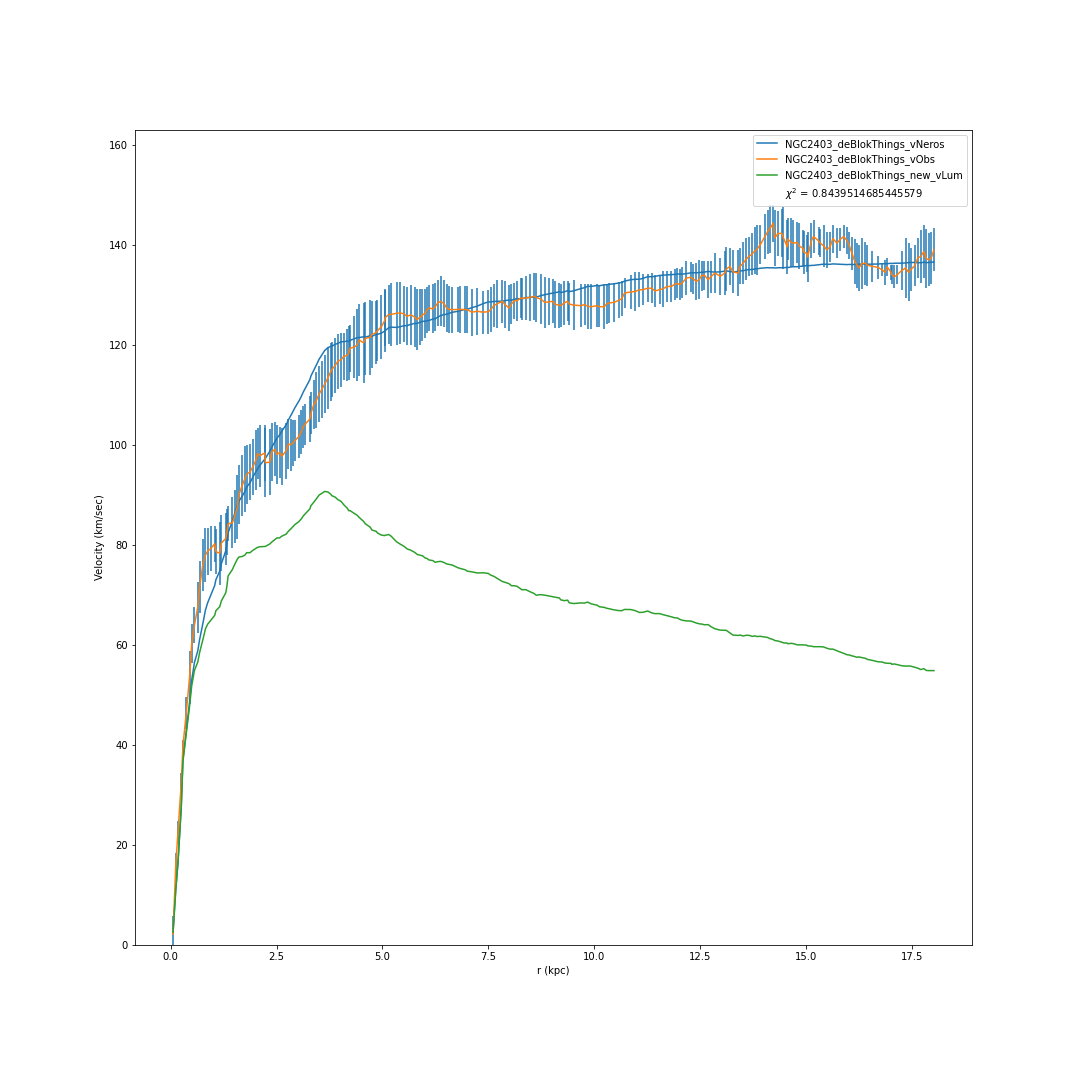
\includegraphics[width=0.95\linewidth]{figures/NGC2403_deBlokThings_XueSofue}
   % \caption{ }
  \end{subfigure}%%
  \caption{ RCFM fit to  NGC 2403  rotation curve data and   baryon model from  \citet{Blok1})}  \label{fig:NGC2403RCFM} 
\end{figure}



  S. McGaugh's notes one such paradox when he asks   ``Why is the luminous tail wagging the dark matter dog,  if dark matter dominates dynamics ?'' \cite{1999McGaugh,McGaugh2016RAR}. This references the  disk-halo conspiracy;  that knowledge  of 
 the   stellar   disk     determines the spherical dark matter halo \cite{2004ApJ...609..652M}. A   related paradox is the Universal Rotation Curve (URC), which  involves a spectrum of   1,100  rotation curves plotted on the same axes, and normalized by scale-length 
 (See Fig.~\ref{fig:URC}))  \cite{salucci,Persic,1978Rubin,10.1111/j.1365-2966.2007.11696.x}. The URC spectrum   inflects about a median point of the Milky Way's presumed rotation curve,   where galaxies larger than the Milky Way have 
 rotation curves which    inflect down toward the   flat   curves, and galaxies smaller than the Milky Way inflect up toward flat.
 In the dark matter paradigm there is no explanation for  this phenomena, that   the Milky Way is in the middle of such a  spectrum \cite{MCGAUGH2021220}. 

 
 
    


% This paradox    requires fundamental modifications to the classical theory of gravity, because in classical gravity mass accretion rates favor   larger mass concentrations \cite{10.1093/mnras/stt2403}.  However,    these paradoxes disappear if we instead view them as indicative of  frame dependent effects due to  the relative frame of the   Milky Way, imprinted on observations of Doppler shifted spectra. 
 
The   leading   alternative     to dark matter models is   Modified Newtonian Dynamics (MOND) \cite{Milgrom},  and while  the   luminous mass is the only mass   there is   a changing   scale of gravitational acceleration which fundamentally alters gravitational physics \cite{McGaugh_2014}. MOND introduces a new acceleration scale to successfully fit   a large number of spiral galaxies  rotation curves with essentially a single constant acceleration scale \cite{2016Lelli}.
   While MOND fits to galactic rotation curves are competitive with those from dark matter theories, judging by number of free parameters,  goodness of fits and resulting mass-to-light ratios, it is still a modification of the well tested Poisson gravity  \cite{McGaugh2016RAR,2022A&A...664A..40M}. 
   The limitation of MOND is apparent in a few galaxies at well calibrated distances (Cepheid variable stars), where MOND fits require different distances.
  %  {\color{blue}(MOND - when is distance a free parameter? in RAR apparently as well, thouhg they slipped that right past me until now )}  {\color{blue}(Dark Matter - how many free parameters in DM models?answer: variously 2-4)}
  
  We present a new paradigm, in which these paradoxes are resolved by  attributing excesses in Doppler shifted spectra to  a frame-dependency  due to our Milky Way.   We identify photometric measurements as Lorentz scalars which are agreed upon between frames, given a reliable distance estimate,  and Doppler-shifted spectra as a part of  Lorentz 4-vectors which must transform appropriately.    We will assume that the luminous mass is the only mass, and that   test particle velocities in  orbit around   the galactic centers are those expected from  the Keplerian estimates from  total light.   
    Previously, the role of relative
     galaxy curvature  in this problem was obviated 
       by  Galilean subtraction of   gravitational red-shifts at the  large $r$  limit of the data \citep{MTW}. 
    
    
    Previous attempts to extend MOND into the relativistic regime have given rise to  new theories of gravity  \cite{PhysRevD.70.083509,doi:10.1142/S0217751X0703666X,Famaey2012}, but the approach we propose is more conservative as it does not modify gravitational theory but rather introduces a heuristic technique for mapping between galactic gravitational frames.  Further, the approach we present transitions the  MOND paradigm of changing acceleration scales to the relativistic concept of  changing relative  curvatures. We show in this paper that this new approach  preserves the fitting successes of MOND, but   increases accuracy  for some notorious problem galaxies. 
 From this perspective,   MOND's  roughly constant acceleration scale is a   characterization of the role of the Milky Way on our observations.  We demonstrate the success of this new approach by fitting   a sample of 175 galaxy rotation curves previously fitted by the MOND   and an extension of MOND called RAR (Radial Acceleration Relation) \cite{McGaugh2016RAR,2016Lelli,McGaugh_2014,Li_2018}. 
  
     
  At this time, there are many problems in   the concordance model of   cosmology which are attributed to dark matter \cite{2010dmp..book.....S,Tully:2014gfa,Naidu_2022}, but in
 this paper we address only this  one, as it is the simplest.  
 This paper  is organized as follows;
{\bf Section \ref{sec:dos}} constructs  the new rotation curve  fitting formalism, 
{\bf Section \ref{sec:data}}   describes  the data  we use, 
 {\bf Section \ref{sec:analysis}}   discusses our results, 
 and  {\bf Section \ref{sec:conclu}}   discusses implications and future tests.   
  
  
 \begin{figure}[h!]
     \centering
     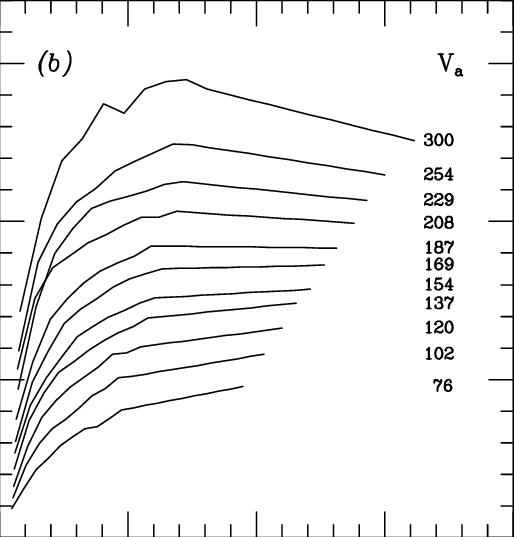
\includegraphics[width=\linewidth]{The-universal-rotation-curve-of-spiral-galaxies-at-different-luminosities-and-velocities}
     \caption{\emph{Universal Rotation Curve spectrum from Ref.\citep{salucci}, Used with permission}}
     \label{fig:URC}
\end{figure}
  

  
    

%%%%%%
%%%%%%%%
%%%%%%
%%%%%%%
%%%%%%
%%%%%%
\section{ Rotation Curve Fitting Models  \label{sec:dos}}
 
 
 \subsection{Dark matter rotation curve fitting formula}
 
  

 The   dark matter rotation curve formula   is of the form

 \begin{equation}
v(r)^2_{rot}  =  v(r)^2_{lum}  +  v(r)^2_{dm},   
\label{eq:zonte1}
\end{equation} 

  where terms in $v(r)_{lum}$ are the Keplerian velocities due to the luminous mass,  $v(r)_{dm}$ are the velocities attributed to  dark matter, and 
  terms in $v(r)^2_{rot} $ are the dark matter model prediction which are fitted to the flat rotation curve data
  $v_{obs}$. All velocities are assumed to be circular orbits, in the plane of the stellar disk,  about the rotation axis of the galaxy at  $r=0$. 
  
 Doppler shifted spectra data  $\omega'(r)$ give 
terms in  $v_{obs}$   by a 
 Lorentz boost between inertial frames, 
   

 \begin{equation}
 \frac{v_{obs} }{c}=
\frac{  \left( \frac{\omega'(r)}{\omega_o}\right)^2 -  \left( \frac{\omega_o}{\omega'(r)} \right)^2 }{  \left( \frac{\omega'(r)}{\omega_o}\right)^2  +  \left( \frac{\omega_o}{\omega'(r)}\right)^2 }, 
\label{eq:modelLumA}
\end{equation} 

  for the  $\omega_o$   the
  characteristic lab  frame frequencies, and terms in $c$   the constant vacuum light speed.  
  
  
 %%%%%%%%%%%%%%%%%
 %%%%%%%%%%%%%%%%%%
%%%%%%%%%%%%%%%%%%%%
Terms $v_{lum}$, in Eq.~\ref{eq:zonte1},    come from observations of total light  (photometry) interpreted by 
the  Poisson equation.  
Population Synthesis Models (PSM)  give   mass-to-light ratios  $\gamma_i$, and associated Keplerian   orbital velocities 
  
   \begin{equation}
v(r)_{lum}^2 = \gamma_b v(r)_{bulge}^2 +  \gamma_d v(r)_{disk}^2 + v(r)_{gas}^2.    
\label{eq:zonte3}
\end{equation} 
  
 Terms in     are   mass-to-light ratios for the stellar bulge $\gamma_b$ and disk $\gamma_d$ respectively.  Gas fractions $v_{gas}$ are calculated from surface density profiles of HI  with the formalism given in  \cite{1983MNRAS.203..735C}, and do not require  a mass-to-light ratio.  
  

The quadratic velocity sums (Eq.~\ref{eq:zonte1} and Eq.~\ref{eq:zonte3})  represent  sums of the  gradients in the gravitational potentials in radius, as
 

\begin{equation}
 \frac{\partial \Phi(r)_{lum}}{\partial r}    =\frac{v(r)_{lum}^2}{r},  
    \label{zoochance1}
\end{equation}

  
for each mass component obeying the Newtonian central     force law for a gravitational potential like

\begin{equation}
      \Phi(r)  = -G \int d^3r'  \frac{ \rho(r') }{r-r'}.
      \label{eq:Newt}
      \end{equation}

The gravitational potential solves Poisson's equation

\begin{equation}
\nabla^2 \Phi(r)_{lum}  = 4\pi G \rho(r),     
    \label{whatsgood}
\end{equation}

 where terms in  $G$  are Newton's   gravitational constant, and 
$\rho(r')$  the mass density. 
  



\subsection{New rotation curve fitting formula}

 The  new 
frame-dependent Rotation Curve Fitting Model (RCFM)   relies on 
replacing the gradient in the potential    $v(r)^2_{dm}/r$  attributed to   dark matter,  with  Lorentz-type transformations between galaxy frames.  Like MOND, We will assume baryonic mass is the only mass in this problem, but different from MOND we will not interpret  terms in Doppler shifted spectra  $v_{obs}$ as physical rotation velocities, but rather as excesses in spectra shifts due to relative galaxy frames. 


Fundamental to this approach is the early identification of  luminosity   as a Lorentz scalar, and Doppler shifted spectra encapsulated in  
  $v^2_{obs}/r$ as part of a 4-vector. Lorentz scalars are agreed upon by both frames under a reliable indicator of  distance (Cepheids, Tip of the Red Giant Branch). 
We  will also assume that the contributions to  Doppler shifted spectra from  relative frame  motion ($v_{lum}$) can be  decoupled from those from relative curvature roughly as in Eq.~\ref{eq:zonte1} \cite{Jack,Cisn}. 



 
 
   
   The new rotation curve fitting model (RCFM) we propose  replaces dark matter in Eq.~\ref{eq:zonte1} with a series of Lorentz type transformation $v_1$ and $v_2$,
   

\begin{equation}
v(r)_{rc}^2 =  v(r)_{lum}^2+\alpha \kappa^2 v(r)_{1} v(r)_{2},  
\label{eq:zonteLCM}
\end{equation}  

  In what follows, all   terms  can be assumed to  be functions of radius except the model's free parameter $\alpha$,  which is single valued for each galaxy fitted, and the speed of light $c$.  
  
  Terms in 
$\kappa$  are   ratios of the baryonic gravitational potentials

 \begin{equation}
\kappa=\frac{\Phi_{gal}}{\Phi_{mw}}, 
\label{eq:kappa2}  
\end{equation}  

 for $\Phi_{gal}$ the    Newtonian gravitational potential of the galaxy being observed, and $\Phi_{mw}$ that of  the Milky Way.  
 
 
 Since    excesses in Doppler shifted spectra
  are     part of  a Lorentz 4-vector, they    must transform in a Lorentzian sense. We haved searched the parameter space of hyperbolic transformations of Rindler's  accelerated  frames \cite{Cisneros:2013vha,Cisneros:2014fea,Cisneros2015,Cisn2016}, and find the best fit function for $v_1$  is

 
 
   \begin{equation}
       v_1 = \sinh \zeta, 
       \label{eq:hyperbolica}
   \end{equation}
 
 for a rapidity angle $\zeta$,  defined by the    Lorentz exponential  term  
  
   
     \begin{equation}
     e^{\zeta}=  \frac{\omega_{mw}}{\omega_{gal}}  =\sqrt{\frac{g_{tt}|_{gal}}{g_{tt}|_{mw}}},
      \label{eq:gravRS}
    \end{equation}
    
 for  clock terms $g_{tt}$   defined in the   weak field Schwarzschild limit  \cite{Hartle} as, 
 
  \begin{equation}
      g_{tt}= -( 1 - 2\Phi/ c^2).
      \label{clocktime}
  \end{equation} 
  

The best fit function for  $v_2$ is 

\begin{equation}
v_{2} =  \cosh \tau, 
\label{eq:hyperbolico}
\end{equation}


 
 
  for a rapidity angle $\tau$ defined by the    Lorentz exponential  term  
  
 
\begin{equation}
    e^{\tau}=   e^{(\zeta+\eta)/2}.
\end{equation}
 
Terms in $e^\eta$ represent the  flat field-frames with the
Lorentz exponential  

\begin{equation}
    e^{\eta}=\frac{\omega_{l}}{\omega_o}= \sqrt{\frac{1+\beta}{1-\beta}},
    \label{eq:flat}
\end{equation}  
     
which comes from estimates of the Keplerian velocities due to luminous mass
$\beta = v_{lum}/c$, rewritten as the expected      frequency shifts $\omega_{l}$      by a inertial frame Lorentz boost   

 \begin{equation}
 \frac{v_{lum} }{c}=
\frac{  \left( \frac{\omega_{l}}{\omega_o}\right)^2 -  \left( \frac{\omega_o}{\omega_{l}} \right)^2 }{  \left( \frac{\omega_{l}}{\omega_o}\right)^2  +  \left( \frac{\omega_o}{\omega_{l}}\right)^2 }. 
\label{eq:lumlorentz}
\end{equation} 
 
 
  Lorentz exponential terms (Eq.~\ref{eq:gravRS} and Eq.~\ref{eq:flat})
  are    identified  as the  frame field relationships   by  comparing 
     the  Lorentz transformation in  Eq.~\ref{eq:modelLumA} with 
 its   hyperbolic form \cite{rindler2013essential} 


     \begin{equation}
         \frac{v}{c} = \tanh \theta = \frac{e^\theta - e^{-\theta}}{e^\theta + e^{-\theta}} .   
         \label{boost}
     \end{equation} 

 
 
Heuristically, terms in  $v_1$ map the gravitational frame of the observed galaxy onto that of the Milky Way, and  terms in $v_2$  then  map from  that   curved 2-frame  (Eq.~\ref{eq:gravRS}),  to  the flat 2-frame where we make observations. 
  That this second transformation  is necessary is evidenced by the local constancy of the speed of light. Viewed as    Rindler's accelerated coordinates\cite{MTW,Wald, rindler2013essential}, 
     $v_1$   is  timelike   and $v_2$ is spacelike.
By use of Eq.~\ref{eq:flat}, we    assert  that Keplerian rotation curves are     the best estimate of flatness, since dark matter is not required to  reproduce the rotation curve of our Solar System.
 
    
  
 
  
 
 
%%%%%%
%%%%%%%
%%%%%%
%%%%%%%  
%%%%%%
%%%%%%%  
\subsection{Synchronizing the gravitational potentials \label{sec:gravDets}}

  
    
    

 
Lorentz exponential terms in  $v_1$ and $v_2$ are parametrized with ratios of  the    Schwarzschild gravitational redshifts

\begin{equation}
       \frac{\omega_1}{\omega_2}  =\sqrt{\frac{g_{tt}|_{P2}}{g_{tt}|_{P1}}} =\sqrt{\frac{|\xi^t\xi_{t}|_{P2}}{|\xi^t\xi_{t}|_{P1}}}.
      \label{eq:grav}
    \end{equation} 
    
Eq.~\ref{eq:grav} is    intended to represent the change in a photon energy due to  moving from point $P1$ to $P2$,  in the same manifold \cite{Wald}.   This is based on the conservation properties of the Killing field. 


To  extend this formalism   to connect 
  two distinct gravitational manifolds, we consider  Wolfgang Rindler's statement that        ``the center of each galaxy provides a basic local standard of nonacceleration ... so then can be treated like a local inertial frame relative to its own center.''\cite{rindler2013essential}.
   So, to compare two   galaxies inertially  we rely on synchronizing their respective   centers, which means aligning their integrated potentials from the place where all galaxy clocks read zero   $g(R_s)_{tt} = 0$, at the event horizon $R_s$. 
   Terms in 
  $g_{tt}(r)$ are  parametrized with  the Newtonian  gravitational potentials   Eq.~\ref{clocktime}. 
  
 
   
 Usually, gravitational potentials of galaxies are compared from the zero at  the large $r$ limit,  where  $\Phi$ is assumed  to go to zero. 
 In calculations, this amounts to integrating the potential from large $r$ and  zero potential, in to the small $r$ limit where the potential reaches a negative maxima at   $r\approx 0$. 
This procedure  ensures   energy goes to zero at infinity, which is consistent with a picture of a globally flat embedding space.   However, since 
  the external environments of galaxies at the large $r$  limit of the data appear to be  extremely complicated  and diverse (ie. nonflat) \cite{Pomarede:2020pme,Hoffman:2017ako},   we will instead compare galaxies from potentials integrated from  zero at the   small $r$ limit, out to the maximum radius observed. This means that all our potentials are calculated with respect to the same zero of the potential, and we do not require them to be embedded in a globally flat spacetime.
   
 
  

 \begin{equation}
     \Phi  =    \int_{inner}^{outer} \vec{F_r}\cdot\vec{dr}.
      \label{eq:Newt2}
      \end{equation}
 
 

   
 Potentials calculated in this way still obey the central force law for test particles moving in circular orbits in Eq.~\ref{zoochance1} and Poisson's equation Eq.~\ref{whatsgood}.
   
  
\subsection{  Geometry Considerations  }\label{GeomSphere}
  
   Population synthesis models commonly assume spherical symmetry for the 
  stellar bulge, gas halo, but use axial symmetry to model     the stellar disk \cite{1954AJ.....59..273S}.
 However, it is a common calculational  tool to use spherical symmetry for the entire luminous mass integrated potential \cite{2022A&A...664A..40M,PhysRevD.70.083509}, because numerical integration of the thin disk is  computationally intensive,  requires assumptions of  boundary conditions,   relevant physical scales,  etc. and therefore adds extra free parameters to the problem \cite{2011A&A...531A..36H}.  
 We will use the spherical approximation here  because  the simplest metric for this situation is that of 
 Schwarzschild. 
 
Gravitational potentials calculated for  a spherically symmetric  geometry will 
  merge to those calculated for an exponential disk  at lengths greater than one-third of the exponential scale-length of the disk $R_e$, ie.  $r> R_e/3$\cite{Chatterjee}, where dark matter effects becomes important \cite{1985ApJAlbada}. 
However, 
    in the inner region of a galaxy $r< R_e/3$,  the spherical assumption will 
    overestimates the potential of a thin disk by $\approx   50\%$, see Fig.~\ref{fig:my_geom}.  We note that   the mass in the inner $1/3$ of the stellar disk seems to be where our RCFM fits   sets the mass-to-light ratios. For physical interpretation, we divide all mass-to-light ratios for the disk by a factor of 2. \textcolor{purple}{AR: why divide by two?}
  
  
  \begin{figure}
    \centering
    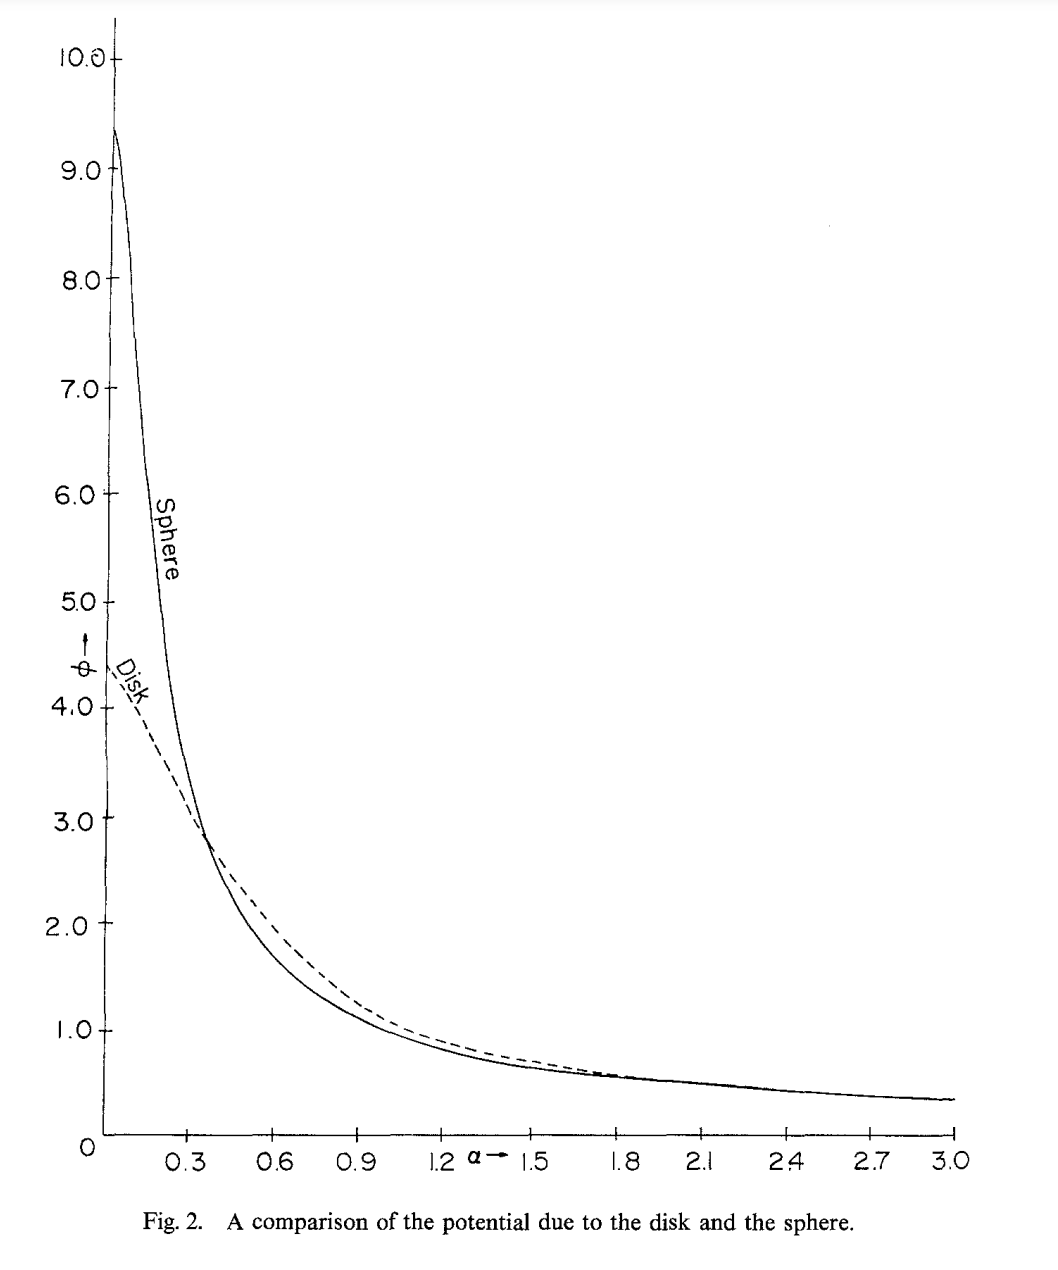
\includegraphics[width=\linewidth]{figures/Chatterjee_SphereDisk.png}
    \caption{ $\alpha = r/R$, for $R$ the radial extent of the stars \cite{Chatterjee}. Ask permission.}
    \label{fig:my_geom}
\end{figure}  
    
      
    

%%%%%%
%%%%%%%
%%%%%%
%%%%%%%
%%%%%%
%%%%%%% 
%%%%%%
%%%%%%
%%%%%%%  
%%%%%%
%%%%%%%  Do analysis on N7814 and N891
%%%Compare Fraternali y DM.
%%%%%%%
\section{Data \label{sec:data}}
 
 \subsection{SPARC Galaxies}
 We fit the Spitzer Photometry and Accurate Rotation Curves (SPARC) dataset  of  175 nearby galaxies with extended rotation curve data from atomic hydrogen (HI)  and H-$\alpha$ \cite{2016Lelli}. 
 HI provides the most reliable
 rotation curves because it is dynamically cold, traces circular orbits, and can be observed several effective radii past the stellar disk. 
 This sample of rotationally supported galaxies   spans the widest range of masses and morphologies currently available. 
 
These galaxies are  accompanied by model rotation curves representing   the  luminous mass components for each galaxy,  from   Spitzer Photometry in the 
   near infrared  at 3.6$\mu m$ interpreted in Poisson dynamics. 
   Near infrared  is  currently believed to be the best tracer of stellar mass   in population synthesis models (PSM) \cite{10.1093/mnras/sty3223}.  PSM, at this wavelength,   give mass-to-light ($\gamma_i$) ratios which are almost constant, independent of star formation history \cite{BelldYong,10.1093/mnras/sty3223}. Luminous mass rotation curves are reported in the SPARC database with all $\gamma_i=1$ in units of $M_{\odot} / L_{\odot}$   at 3.6$\mu m$. 
   PSM rely upon a complex  suite of  assumptions regarding galaxy evolution, metallicities and initial mass functions  \cite{BelldYong,10.1093/mnras/sty3223}, and are underconstrained precisely because rotation curve data produced the dark matter problem.   
   
     Gas fractions $v_{gas}$ are calculated from surface density profiles of HI  with the formalism given in  \cite{1983MNRAS.203..735C} and scaled 
     a factor 1.33 to account for cosmological helium abundances.  Contributions from molecular gas are ignored   because CO data are not available for most SPARC galaxies. 
     Error on these velocities is estimated at $20\%$ \cite{2016Lelli}. 

   
   
     All terms in $\Phi(r)$ (Eq.~\ref{clocktime})  are    integrated from estimates of the baryonic mass as described in Sec.~\ref{sec:gravDets}, as reported  in the      SPARC  library at \url{http://astroweb.cwru.edu/SPARC/}.    

 
   

  
%ASK STACY and compare to ours
 %Their final science sample is made of 153 galaxies.
 


%%%%%%
%%%%%%
%%%%%%%
\subsection{Milky Way}\label{MWselect}


The rotation curve fitting model presented here requires a static choice for the baryon distribution of the   Milky Way (MW). 
Mass-modeling of the MW is an under-constrained problem, due to     observing from       within  the disk  \cite{1991ARA&A..29..409F}.
 Beyond our position at 8 kpc, the data is very 
 noisy, see  Fig.~\ref{fig:mwSofue}.  
 
 
 We test the RCFM   using two different, static MW choices; 
   a hybrid model combined from  \citet{Xue}, 
  \citet{Sofue}, \cite{sofue2009unified}, and 
  a model from  \citet{McGaugh_2019}. The Sofue and Xue MW are derived from the same data and same model constraints.     They are combined because the MW from  \citet{Sofue} covers a range of   $[0,20]$ kpc, and   \citet{Xue} from
  $[20,60]$ kpc. 
  
   The  two Milky Way models vary in their underlying assumptions about the fundamental structure and gravitational behavior of the Milky Way. For example, McGaugh \cite{McGaugh_2019} assumes a galactic bar at the center and thus does not include velocity data of the inner 5 kpc of the Milky Way.  Whereas, the Xue-Sofue MW peak velocity is   at around $94$ parsecs, versus that for  the McGaugh MW   at  approximately  $6.55$ Kpc due to the   bar  \cite{McGaugh_2019}. See Table~\ref{tab:MWcompare} for more information.
  
  
  
Both MW models come from    deconvolving the   luminous mass of the stellar disk  from the rotation curve data  using either MOND or dark matter models. 
   
   
   

 
    
  
  
  
  \begin{table*}[]
      \centering
       \caption{Comparison of the two Milky Way models used in this paper}
      \label{tab:MWcompare}
       \begin{tabular}{|c|c|c|c|c|c|}
      \hline
        Milky Way Model & Photometry                        & Model dependence  & Rotation Curve data & scale radius bulge &$\gamma_{bulge}$\\
 \hline
Xue-Sofue     
&  2.2$ \mu m$
& NFW \cite{1996ApJ...462..563N}     
&SDSS DR6  \cite{Xue}       
& $Rb = 0.5$ kpc    
&$  7.1 M_\odot /L_\odot$  \\
  \hline
 McGaugh       
 & 3.6$\mu m$ 
 &MOND \cite{Milgrom}
 & CO data  \cite{2006ApJ...641..938L}                            
 &  N.A.  bar assumed
 & N.A. bar\\
         \hline
      \end{tabular}
     
  \end{table*}
  
  \begin{figure}
    \centering
    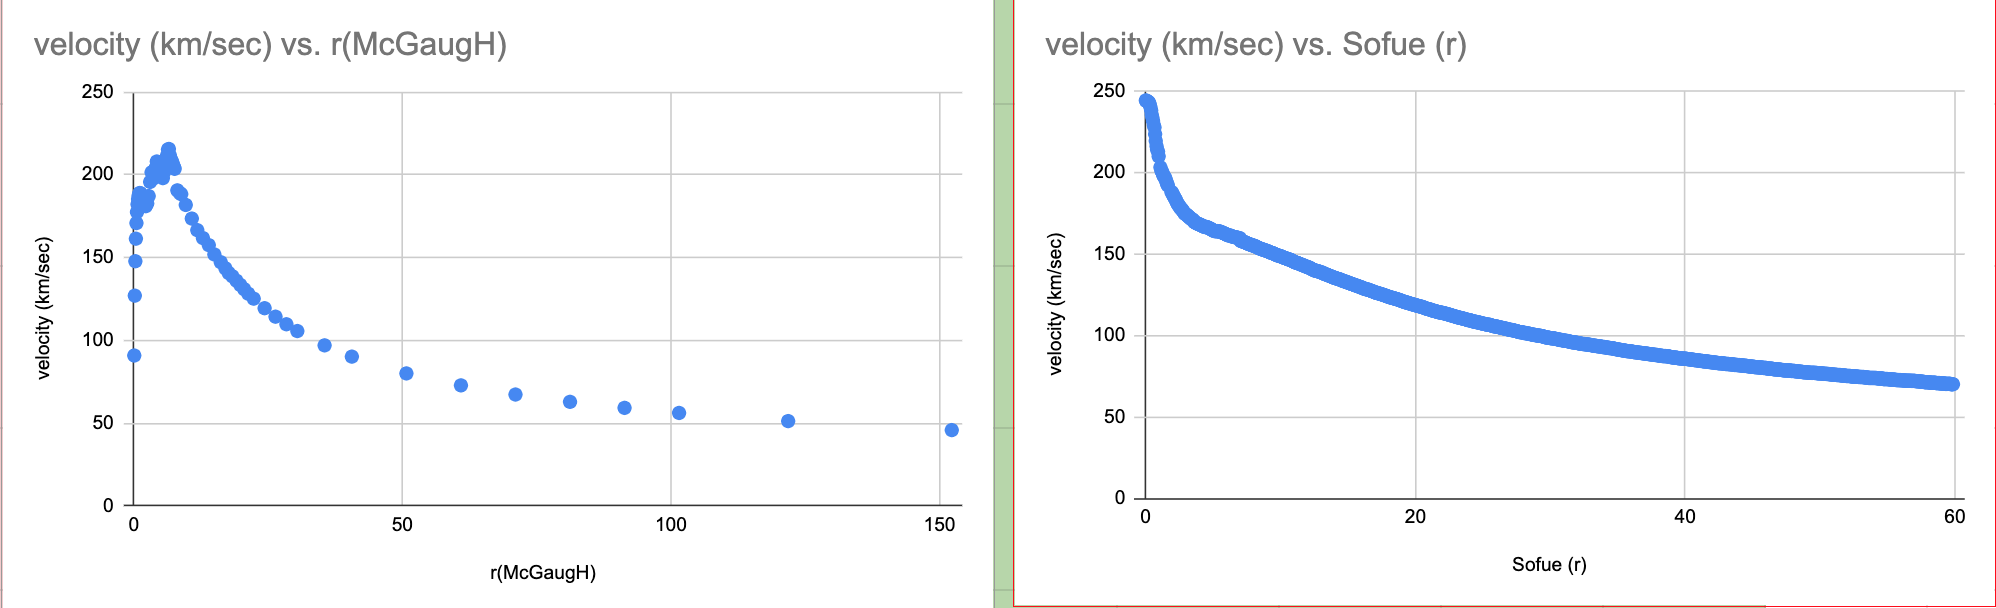
\includegraphics[width=\linewidth]{figures/MWXueSofueVMcGaugh.png}
    \caption{[REMAKE GRAPHS:  both MW are on one graph.] Milky Way rotation curves
   from Xue-Sofue and McGaugh \cite{sofue2009unified}, \cite{McGaugh_2019} }
    \label{fig:mwSofuevMcGaugh}
\end{figure}

 \begin{figure}
    \centering
    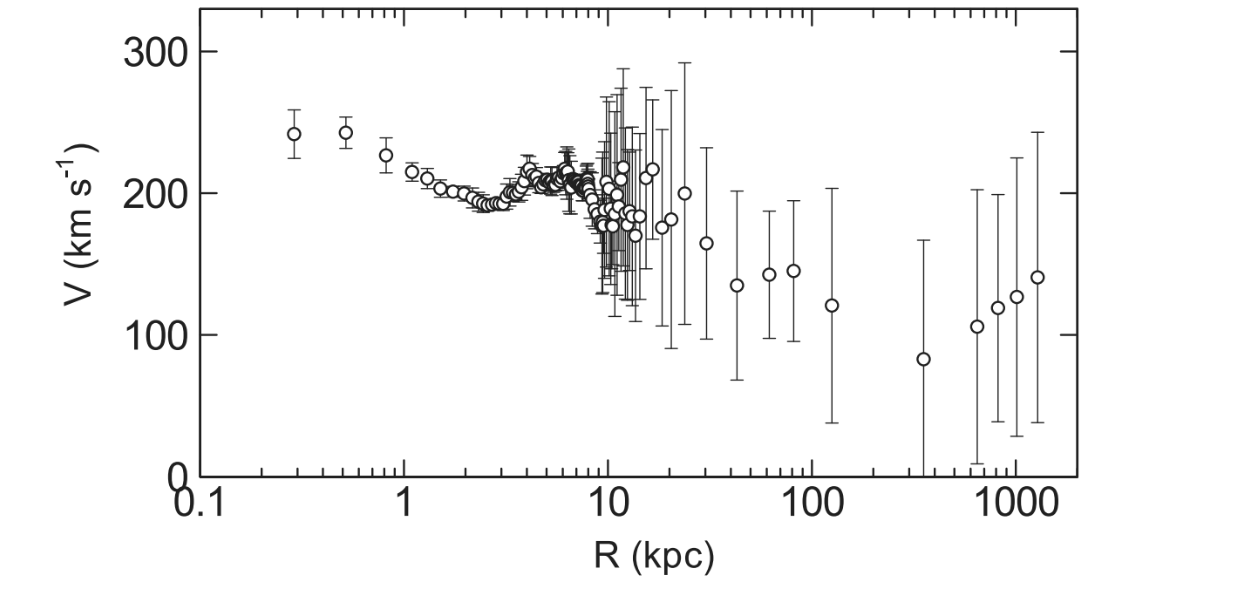
\includegraphics[width=\linewidth]{Sofue_MWtoLGData}
    \caption{ Milky Way rotation curve data from radio signals and SDSS CO star line shifts  \cite{Sof11}. Ask permission.}
    \label{fig:mwSofue}
\end{figure}

%Sofue: We included the circular velocities from an SDSS blue stars analysis by Xue et al. (2008; their model 1) by correcting for a systematic difference in the veloc-ities of about 20 km s1, due to our V0 = 200 km s1 instead of their 220 km s1.
%ugggh. have to look at the first two papers to see what assumptions they make. 
%We decomposed the newest rotation curve into a de Vaucouleurs bulge, an exponential disk, and an isothermal dark halo (Sofue et al. 2009).
%OBS METHOD: 
%An inner rotation curve was obtained by a terminal-velocity method applied to radio line observations
% An outer rotation curve was obtained by combining the CO star line velocities and the optical distances
%and by the HI disk-thickness method
%de Vaucouleurs bulge of mass Mb = 1.8 1010 Mˇ with a scale radius of Rb = 0.5 kpc, an exponential disk of mass Md = 71010Mˇ with a scale radius of Rd = 3.5 kpc,
%In the inner Galaxy at R .10 kpc, the rotation velocity is predominantly determined by the bulge and disk contributions, and R < 0.5 kpc it is almost determined by the bulge alone.


  
%   \begin{table*}[h!]
%      \centering
%      \begin{tabular}{|c|c|c|}
%      \hline
%        Author & Position of the Solar system   &  scalelength disk\\
%        \hline
%        Sofue \cite{sofue2009unified,10.1093/pasj/61.2.153,Sof11}   & 8 kpc &\\
%             \hline
%        McGaugh\cite{2021DDA....5240103M} & &\\
%         \hline
%        Klypin&&\\
 %        \hline
%        Enbang Li&&\\
%         \hline
%      \end{tabular}
%      \caption{MW}
%      \label{tab:my_label}
%  \end{table*}
  
 

 


 








\section{  Analysis and Results \label{sec:analysis}}
 
 

 
 
 


{\color{blue}\emph{COMMENT MEAGAN: We'll want a better title, and this is basically a first draft.  Also, this probably isn't the right order to do things in. Maybe we should first address which galaxies we analyze, then the actual fitting, then interpreting $\alpha?$} }


\subsection{fitting procedure}



To fit galaxies in the SPARC sample,  the fitting procedure is as follows.   First,  a       Milky Way model must be chosen (see Sec.~\ref{MWselect})  and the data  read in as $v_{lum}(r)$ for a series of measurements in radii. The galactic potential is computed as per Eq.~\ref{eq:Newt2} by numerically integrating

\begin{equation}
\Phi(r) = \int_{inner}^{outer} dr \frac{ 
v(r)^2_{lum} 
}{r}.
\label{nowthen}
\end{equation}

Once the MW potential is calculated, it remains static for the rest of the fitting procedure.  

The data for the   galaxies being observed include several pieces of information: the rotation curve velocities $v_{obs}(r)$ from Doppler shifted spectra, the uncertainty on that measurement $v_{err}(r)$, and the components of the luminous mass interpreted as orbital velocities,  $v(r)_{bulge}$, $v(r)_{disk}$, and $v(r)_{gas}$. 
To calculate the baryonic potential for the galaxy in question, $v_{lum}(r)$ is first computed   as per Eq.~\ref{eq:zonte3}, for $\gamma_b=1$ and $\gamma_d=1$. The $\Phi_{gal}(r)$ associated with that galaxy   is then computed as in Eq.~\ref{nowthen}.

After the $\Phi(r)$ for the galaxy being studied and the Milky Way have been calculated,   the components must be compared at  matching values of $r$. To match radii, the $\Phi_{MW}(r)$ are calculated at  interpolated   radii as reported in the 
rotation curve data $v_{obs}(r)$ for the galaxy being observed. Any point with a radius larger than the largest radius in the Milky Way model is discarded.

The terms in the RCFM   can then be calculated  to produce the  $v_{rc}$ in Eq.~\ref{eq:zonteLCM}, which is  fitted to the  $v_{obs}$. 

 
%({\color{blue} I'm not sure we need to do all this algebra for them....??? }
%To calculate $v_1$ and $v_2$,   the terms $e^\zeta$ and $e^\eta$ are needed, which we rename for convenience. These are as defined in equations (REF) and (REF)

%\begin{equation}
%    \psi_{curve}(r) = e^\zeta = \sqrt{\frac{1 - %2\Phi_{gal}(r)}{1 - 2\Phi_{MW}(r)}}
%\end{equation}

%\begin{equation}
%    \psi_{flat}(r) = e^\eta = \sqrt{\frac{1 + %\beta_{gal}(r)}{1 - \beta_{gal}(r)}}
%\end{equation}

%Where

%\begin{equation}
%    \beta_{gal}(r) = \frac{v_{lum,gal}(r)}{c}
%\end{equation}

%Then the $v_1$ and $v_2$ terms are the respective hyperbolic functions.

%\begin{equation}
%    v_1(r) = \sinh(\eta) = \frac{\psi_{curve}^2(r) - 1}{2 \psi_{curve}(r)}
%\end{equation}

%\begin{equation}
%    v_2(r) = \cosh((\zeta + \eta)/2) = \frac{\psi_{curve}(r) \psi_{flat}(r) + 1}{
 %   2\sqrt{\psi_{curve}(r) \psi_{flat}(r)}}
%\end{equation}

The RCFM prediction is    assembled as in equation \ref{eq:zonteLCM}, to give a predicted $v_{rc}$ which is fitted to the rotation curve data $v_{obs}$. The fit is then minimized to find the  lowest   $\chi^2$,  using the {\tt scipy.optimize.curve\_fit} utility in Python.

The equations outlined in Section \ref{sec:dos} contain three free parameters that must be determined for each galaxy fit:  the model's free parameter $\alpha$,  and the   stellar bulge $\gamma_b$ and stellar disk $\gamma_d$. 
The mass-to-light parameters   are allowed to vary freely from an initial value of $1.0$, see Eq.~\ref{eq:zonte3}, and the $\alpha$ parameter     from an initial value of $\alpha = 0.01$. 

Reported gas fractions (HI scaled for Helium abundance) are fixed,  though addition of molecular gas could increase mass fractions in the inner kiloparsec of a galaxy   \cite{2004ApJ...609..652M}.





\subsection{Evaluating Goodness-of-fits}

There are two metrics by which rotation curve fits are judged. One, the reduced  $\chi^2$ values can be compared between fits to the same rotation curve data, and 
 two, the resulting mass-to-light ratios from the fit as compared to estimates from PSM. 

The $\chi^{2}$ values for fits shown in Table~\ref{table:M2Light} and Table~\ref{tab:lobes} are remarkably low ({\color{blue} more than twice as small as RAR}), providing confidence in the faithfulness of fits to rotation curve data.  
  While reported error    estimates on rotation curve velocities  have not been standardized across the field~\citep{Blok,Gent},     one can reliably   compare $\chi^{2}$ values  to the same rotation curve data. 
%The functional form of ${v_1}$ and ${v_2}$, the mapped velocities used in fits, had a major effect on $\chi^{2}$ of fits to the training set. The ${v_1}$ and ${v_2}$ functions chosen for use in our model resulted in the lowest $\chi^{2}$ and thus provided fits that described the data with the most accuracy according to that metric.
 In Table~\ref{tab:lobes}  the    average mass-to-light ratios for the entire sample are given for both RCFM and RAR fits ,  in comparison to expectations from PSM \citet{McGaugh2016RAR}. 
    
  
  ({\color{blue}Need divide all Table gamma(disk)s by 2 . Discuss with  Stacy.}  As can be seen in Table~\ref{tab:lobes}, The $\gamma_d$ for the RCFM   are consistent with PSM within the stated error of $ 20\%$ \cite{2016Lelli}.   In Sec.~\ref{GeomSphere}, we discuss adjusting for use of  spherical approximation for the exponential disks for computational reasons. 
  
    
    
    \begin{table}[h!]
        \centering
        \begin{tabular}{|c|c|c|c|c|}
        \hline
        &Model & $\gamma_d$ & $\gamma_b$& $\chi^2_{red}$ \\
        \hline
        \hline
           & PSM \cite{McGaugh2016RAR} & 0.5 &0.7&--- \\
            \hline
            \hline
         &   RAR	 &    0.64 &	0.73  & \\
         \hline
         &  RCFM   &  0.56 &	0.81&\\
           \hline\\
           \hline
        \end{tabular}
        \caption{ Average mass-to-light $\gamma_i$  ratios and reduced $\chi^2$  results from RAR and RCFM fits to the SPARC sample of 175 galaxies. The $\gamma_i$ are in units of  solar mass per solar luminosity $M_\odot/L_\odot$. }
        \label{tab:lobes}
    \end{table}
    
    
   \subsection{Comparing Milky Way Models} 
   
   
    The residuals of fits using different Milky Way models (see Sec.~\ref{MWselect}) were compared to determine which resulted in the best fits.  Histograms of residuals normalized by the error in velocity observations are shown in Fig.~\ref{fig:residual graphs}. 
    
    In all cases, residuals of model fits to observed velocity data followed a narrow distribution centered at zero with a range of +/-3 km/s, albeit with heavy tail features. The behavior of the residuals did not vary greatly between Milky Way models, suggesting that the fitting parameters in our model are robust with respect to differing Milky Way model assumptions. 
    
    A Gaussian fit on residuals from fits using the McGaugh Milky Way model gave a mean of -0.027 km/s, standard deviation of 0.841 km/s and a full-width half-maximum (FWHM) of 1.980 km/s, whereas a Gaussian fit to the residuals from fits using the XueSofue Milky Way model gave a mean of -0.012 km/s, standard deviation of 0.819 km/s and a FWHM of  1.928 km/s. The small values associated with these quantities in both cases provide confidence that our fits matched data closely.
    
    
\begin{figure*}[h]
     \centering
     \begin{subfigure}[b]{0.475\textwidth}
         \centering
         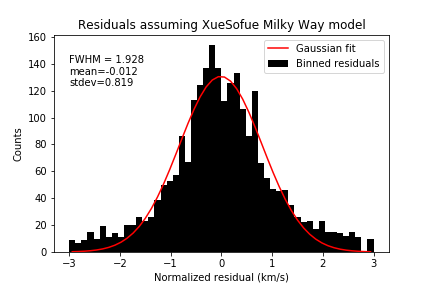
\includegraphics[width=.8\linewidth]{figures/ResidualHist_GaussFit_v1_sinh_v2_cosh_sparc128_newnorm_XueSofue.png}
         \label{fig:XueSofue residuals gaussian fit}
     \end{subfigure}
     \begin{subfigure}[b]{0.475\textwidth}
         \centering
         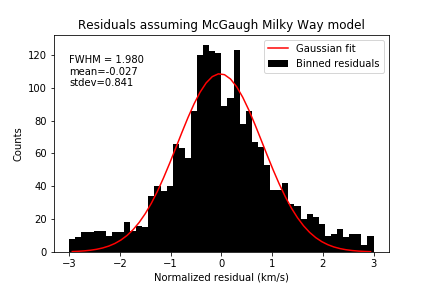
\includegraphics[width=.8\linewidth]{figures/ResidualHist_GaussFit_v1_sinh_v2_cosh_sparc128_newnorm_McGaugh.png}
         \label{fig:McGaugh residuals gaussian fit}
     \end{subfigure}
     \begin{subfigure}[b]{0.475\textwidth}
         \centering
         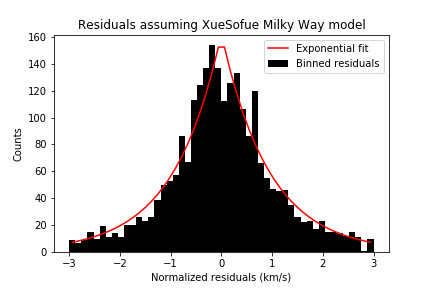
\includegraphics[width=.8\linewidth]{figures/ResidualHist_ExpFit_v1_sinh_v2_cosh_sparc128_newnorm_XueSofue.png}
         \label{fig:XueSofue residuals exponential fit}
     \end{subfigure}
     \begin{subfigure}[b]{0.475\textwidth}
         \centering
         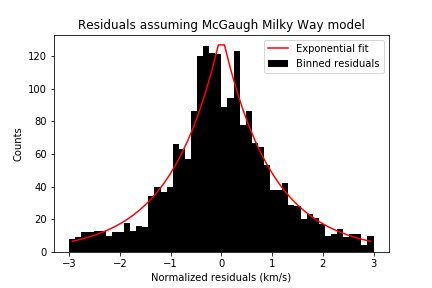
\includegraphics[width=.8\linewidth]{figures/ResidualHist_ExpFit_v1_sinh_v2_cosh_sparc128_newnorm_McGaugh}
         \label{fig:McGaugh residuals exponential fit}
     \end{subfigure}
        \caption{Normalized residuals from fits assuming either XueSofue of McGaugh Milky Way models, fitted to a Gaussian or exponential function. The full-width half-maximums, means, and standard deviations are shown for the Gaussian fits. The exponential fits capture peak and tails in residuals better than the Gaussian fits, suggesting non-Gaussian behavior in the error of velocity observations.}
        \label{fig:residual graphs}
\end{figure*}
Yet, the Gaussian fits did not quite capture the full peak and heavy tails in the residuals. This suggests that there may be non-Gaussian error in the observations of galaxy velocities. To address this, the residuals were also fit to an exponential function shown in Fig.~\ref{fig:residual graphs}. The exponential function captured both the peak and the heavy-tailed behavior of the distributions more faithfully.

% NGC 3198 \cite{1985ApJAlbada} studies this galaxy, which MOND has troubles with. This galaxy has   a thin exponential disk (de Vaucouleurs 1959),(Freeman 1970).  \cite{Toky} mentions that MOND fails to fit NGC 3109, which we fit exceedingly well ($\chi^2 = 0.32$).NGC 2841 is also a problem for MOND
%%%%%%
%%%%%%%%
%%%%%%
%%%%%%%
%%%%%%


 \subsection{ Model Comparisons - individual galaxies}
 \label{results:MtoL}
 
   In this section will  
   compare RCFM results to those from MOND, RAR and dark matter models. 
   McGaugh extended MOND to a new empirical model called the Radial-Acceleration-Relation (RAR)  which maintains the idea of a changing acceleration scale, but arranges the functional dependence in a different way. The RAR represents the  global acceleration relation as
   
\begin{equation}
    g_{obs}=\frac{g_{bar}}{1-e^{-(\sqrt{g_{bar}/g_\dagger})}}
    \label{Eq:RAR}
\end{equation}

for all  terms in $g_i$   the gradient of the potentials as in Eq.~\ref{zoochance1}, specifically 
$ g_{bar} = v_{lum}/r$ represents   the baryons,    $g_{obs}= v_{obs}/r$    the rotation curve data, and terms in  $v_\dagger = 3700 km^2/ s^2 kpc$ represent the changing acceleration scale.  

 
 
 
\subsubsection{NGC 2841}

NGC 2841 is a star dominated spiral galaxy, which   historically, has been regarded as a problematic case for MOND  \citet{Gent}.   RAR   finds a good  fit for this galaxy    after adjusting
the Cepheid   distance of $14.1$ Mpc,  by $1\sigma$,  to $15.5$ Mpc. The RCFM fit is accomplished at the Cepheid distance, 
and has a comparable reduced $\chi^2$ to RAR. The resulting $\gamma_d$   are also commensurate.   The fits are compared side-by-side in  Fig.~\ref{fig:CompareNGC2841}. 

 \begin{figure*}[ht] 
  \begin{subfigure}[b]{0.5\linewidth}
    \centering
    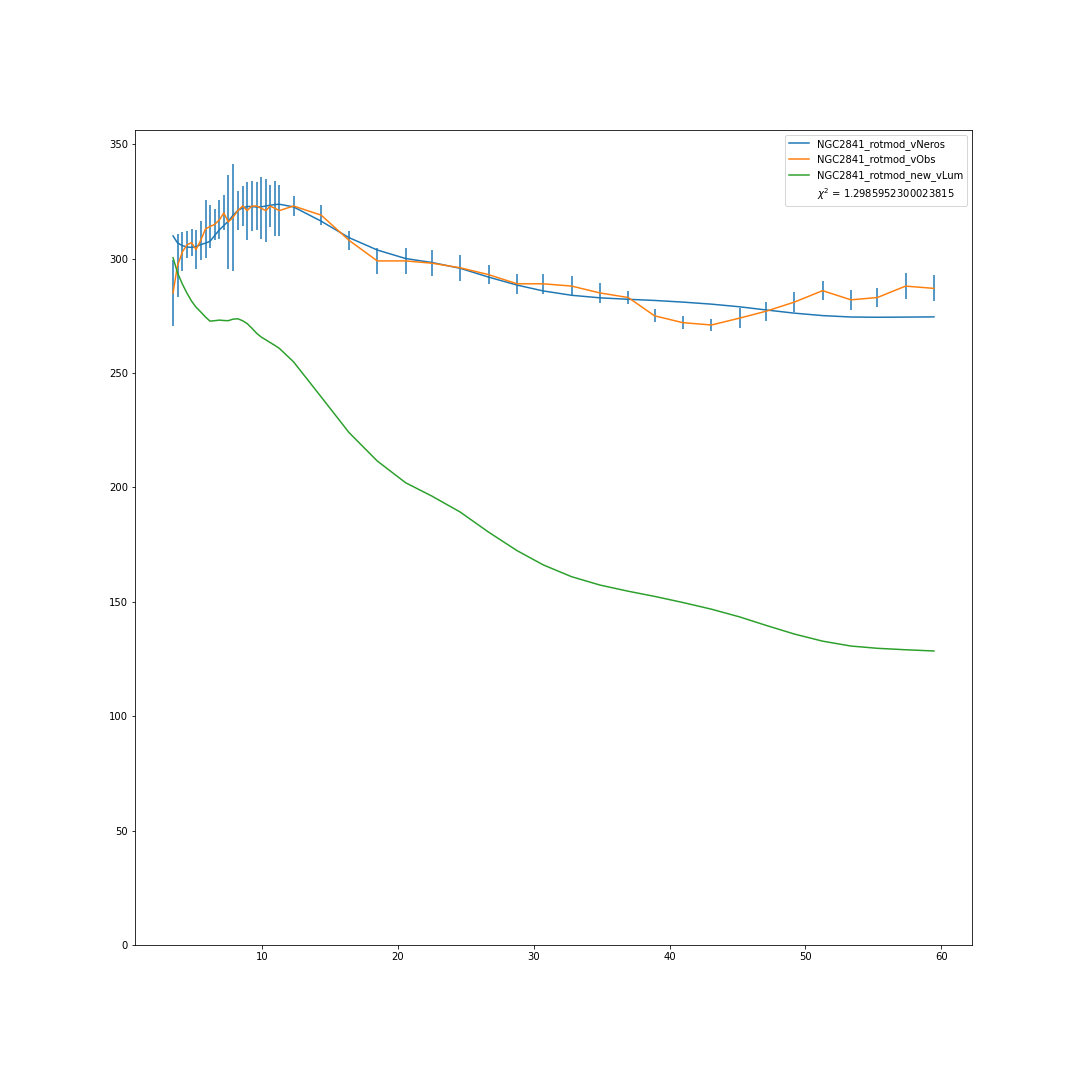
\includegraphics[width=0.95\linewidth]{figures/NGC2841_rotmod_XueSofue.png} 
    \caption{  RCFM fit is the blue line,  Green line is the Keplerian velocity due to  luminous mass estimates, and data points with error bars are the rotation curve data.
  Fitted at the 
    given Cepheid distance $14.1$ Mpc, with resulting mass-to-light ratios of  $\gamma_d = $    and $\gamma_b =1.11$, and  reduced  $\chi^2_\nu = 1.300$.  RUN AGAIN} 
    \label{fig:ngc2841RCFMfit} 
    \vspace{4ex}
  \end{subfigure}%% 
  \begin{subfigure}[b]{0.5\linewidth}
    \centering
    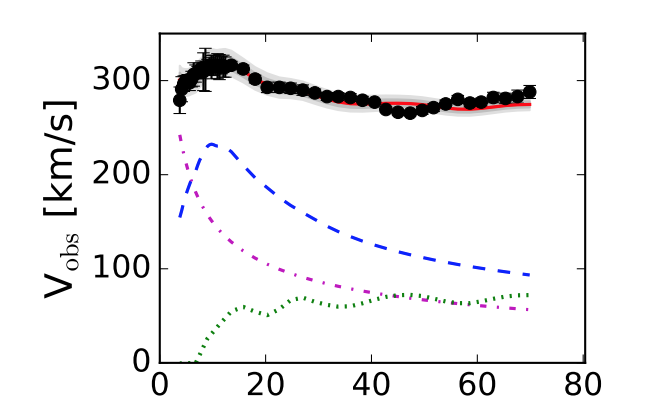
\includegraphics[width=0.95\linewidth]{figures/NGC2841_RarResults_Li2018}
    \caption{RAR fit is the red line, purple line is the bulge, blue is the disk, and green  is the gas \citet{Li_2018}.  ASK PERMISSION TO USE.   Distance parameter fit gives    $15.5\pm 0.7$ Mpc, $\gamma_d =0.81 $ and $\gamma_b =	0.93 $, and reduced $\chi^2_\nu = 1.515$. } 
    \label{fig:2841Li2018Rar} 
    \vspace{4ex}
  \end{subfigure} 
  \caption{Comparison fits to star dominated galaxy NGC2841 }
  \label{fig:CompareNGC2841} 
\end{figure*}

\subsubsection{IC 2574}

IC 2574 is  a gas dominated dwarf galaxy.
Figure \ref{fig:CompareIC2574} shows   fits to this galaxy from  the  RCFM in comparison to  NFW dark matter and RAR fits. 
 RAR finds a good fit to this galaxy    after adjusting
the  distance and inclination by $1-1.5 \sigma$, and their resulting disk mass-to-light 
$\gamma_d  = 0.07$ is  too low to be physical. 
This galaxy is also problematic for dark matter model fits, see Fig.~\ref{fig:Nav17} where the dark matter model significantly overestimates  the rotation curve to 10 kpc, \cite{2017MNRAS.471.1841N}.  
RCFM fit results for this galaxy give  $\gamma_d = 0.553$ , with no adjustment to the reported  tip of the red giant branch distance  of  $3.91$ Mpc. 




 
 \begin{figure*}[ht] 
  \begin{subfigure}[b]{0.5\linewidth}
    \centering
    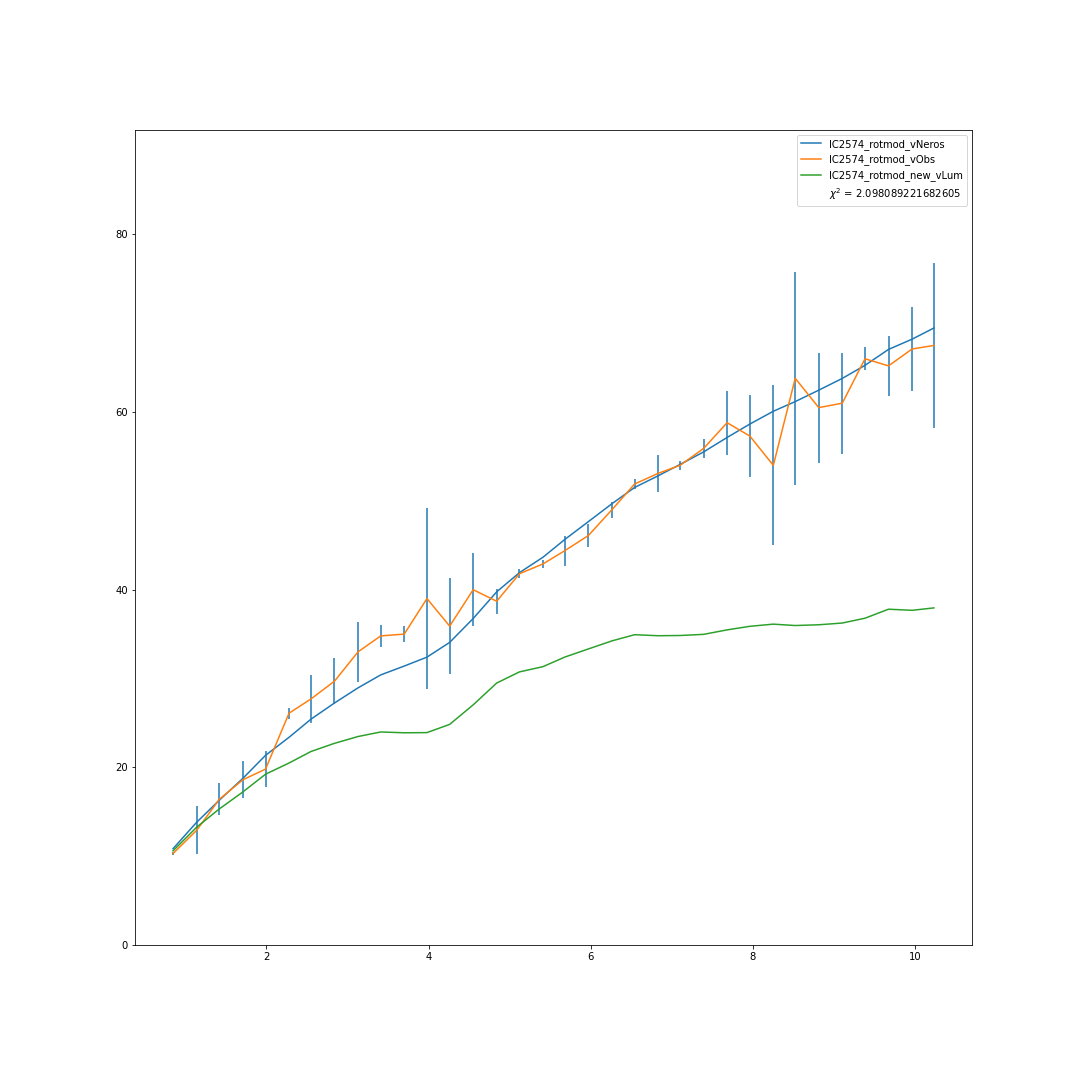
\includegraphics[width=0.95\linewidth]{figures/IC2574_rotmod_XueSofue.png} 
    \caption{  RCFM fit, 
    Fitted at the reported   distance $3.78 ± 0.19 $ Mpc from tip of the red giant branch, $\gamma_d = 1.105 $ (not scaled down by a factor of 1/2 yet), and reduced $\chi^2_\nu = 2.098  $.Lines are as in Fig.~\ref{fig:ngc2841RCFMfit}
    } 
    \label{fig:IC2574} 
    \vspace{4ex}
  \end{subfigure}%% 
  \begin{subfigure}[b]{0.5\linewidth}
    \centering
    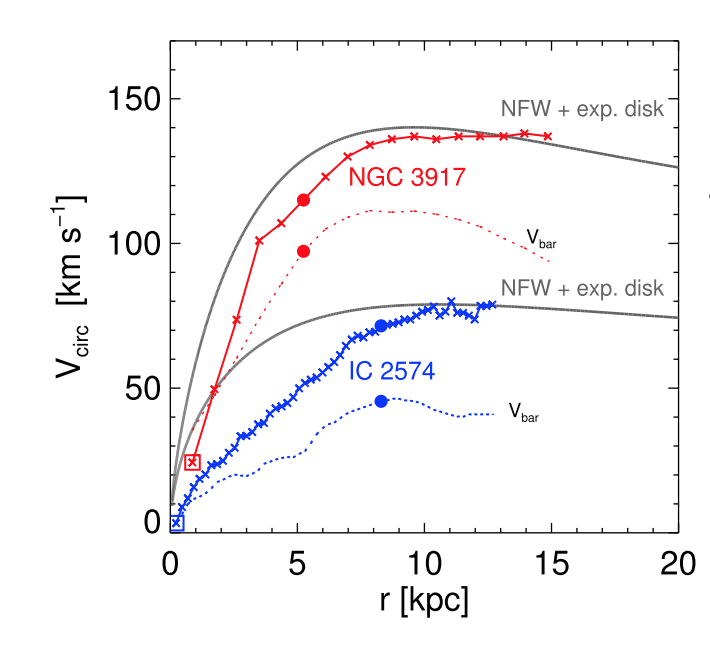
\includegraphics[width=0.95\linewidth]{figures/Navarro2017Fig3.png} 
    \caption{NFW dark matter fit, Figure from \cite{2017MNRAS.471.1841N}, ask permission. Parameter values not reported, but on inspection the dark matter model over predicts central rotation curve velocities.} 
    \label{fig:Nav17} 
    \vspace{4ex}
  \end{subfigure} 
    \begin{subfigure}[b]{0.5\linewidth}
    \centering
    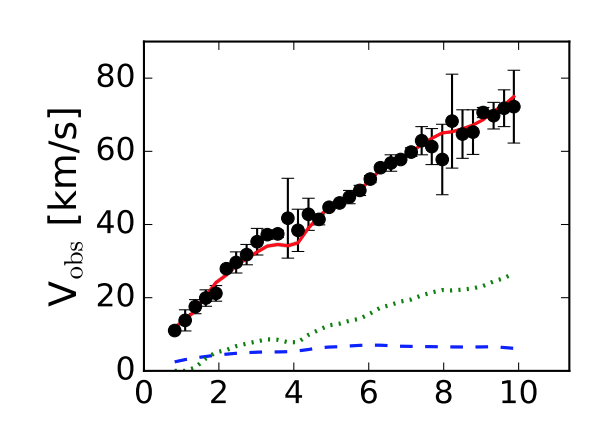
\includegraphics[width=0.95\linewidth]{figures/IC2574_Li.png} 
    \caption{  RAR fit (\cite{Li_2018})   ask permissions. Fit distance parameter gives a distance of $3.77 \pm 0.19$ Mpc, $\gamma_d =0.07 $, and reduced $\chi^2_\nu = 1.44$.Lines are as in Fig.~\ref{fig:2841Li2018Rar}} 
    \label{fig:Nav17} 
    \vspace{4ex}
  \end{subfigure} 
  \caption{ Comparison
fits to   gas dominated IC 2574  }
  \label{fig:CompareIC2574} 
\end{figure*}

\subsubsection{NGC 3198}

  NGC 3198 has historically been a problem  for MOND fits when the distance is a free parameter
\cite{Gent}, as the preferred distance for MOND fits is 2$\sigma$ smaller than that reported from  the most reliable distance indicator, Cepheid variable stars. RAR fits reproduce this distance preference, using a distance of
$ D = 10.4 \pm 0.4$ Mpc  \cite{Li_2018}. With this fit,  RAR gives a reduced
$\chi^2 = 2.057$, and $\gamma_d = 0.77 \pm 0.03$. The RCFM fit to  NGC 3198 at the Cepheid  distance  of 
$13.8$ Mpc, yields  a better reduced $\chi^2 = 1.676$, and mass-to-light ratios of  $\gamma_d = 0.439$.   See Fig.~\ref{fig1super}. 


 


    

   
   
 %TAM (NGC 3198, NGC 7793, and NGC 2976), we do not discuss NGC 7793 and NGC 2976 further, since the MOND fits present the same failures as the dark matter fits (in Newtonian dynamics), therefore we do not consider them as evidence against MOND. We just briefly note that in NGC 7793 the value of the inclination angle fitted by de Blok et al. (2008) is low and presents large variations in adjacent radii, which results in a poorly constrained rotation curve. In NGC 2976 the amplitude of the non-circular motions (Trachternach et al. 2008) is correlated with the amplitude of the fit residuals.
  
    \begin{figure*}[h!] 
    \begin{subfigure}[c]{0.5\linewidth}
    \centering
    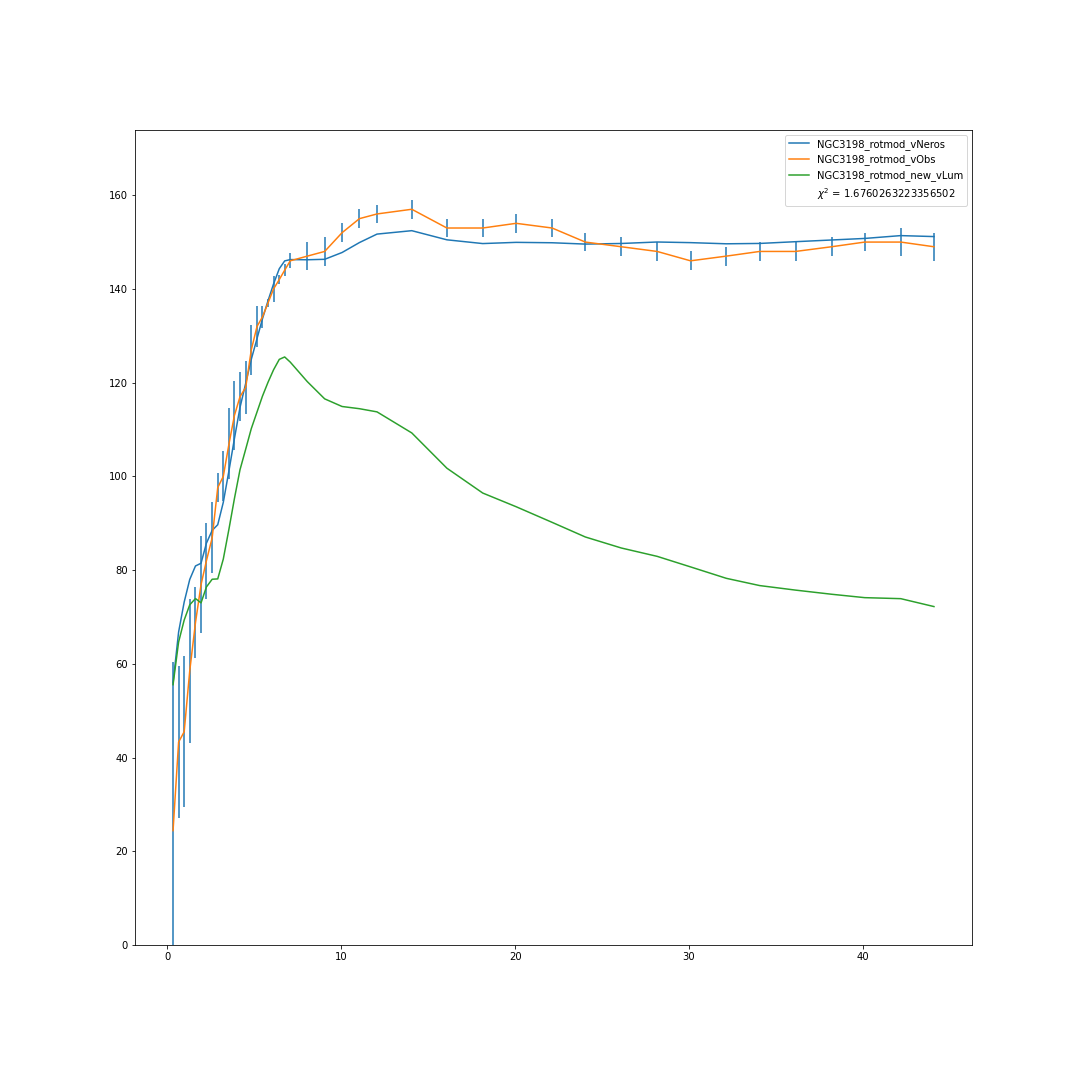
\includegraphics[width=0.95\linewidth]{figures/NGC3198_rotmod_XueSofue.png}
    \caption{RCFM fit blue line, at Cepheid based distance $13.8$Mpc,   luminous mass velocity  green line, reduced $\chi^2  =1.676$, $\gamma_d = 0.878$ (rotation curve data \cite{2016Lelli} }
    \label{fig:NGC3198RCFM} 
  \end{subfigure}%%
  \begin{subfigure}[c]{0.5\linewidth}
    \centering
    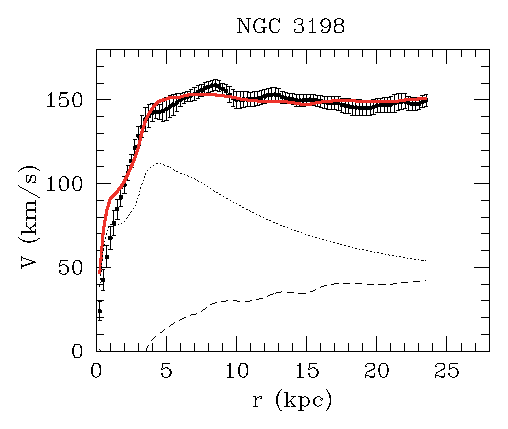
\includegraphics[width=0.95\linewidth]{figures/NGC3198_TAM_aa15283-10-fig7.eps} 
    \caption{ MOND fit red line  , at distance $8.6$ Mpc,    $\gamma_d =  1.01$ in the $3.6 \mu m$ band, $\chi^2=1.56$, $a_0 = 1.2 \times 10^{-8} cm/ s^2$ cm s-2.\cite{Blok1} } 
    \label{fig:NGC3198MOND} 
  \end{subfigure}%%
  \caption{ Rotation Curve Fits   NGC 3198 }
  \label{fig1super} 
\end{figure*}


    \subsubsection{Comparison NGC 7814 and NGC 891}
  
 These two galaxies present an interesting conundrum for both dark matter and MOND models, because they are both presented edge-on, have 'essentially identical rotation curves'', and yet,  are extreme opposites in their morphology,  with NGC 7814 being bulge dominated and NGC 891 almost entirely a disk galaxy. 
 \citet{Frat1} asks, are these rotation curves are actually that identical?
 
 %% remove first point on N891_RotMod , Frat data, and Frat says is from noncircular motions
 
 
 In the context of the RCFM  pardigm, the two rotation are  very similar in magnitude,  but   differ markedly in the inflection  at large radii. 
 NGC 7814 inflects up, and  NGC 891 inflects down.
 In the RCFM paradigm, the inflection of rotation curves indicates   the total galaxy mass in baryons with respect to   the Milky Way.  
 
 However, the RCFM  
fits to these galaxies are successful, see Figures.\ref{fitCompare7814_891}). 
RCFM fits are to the same rotation curve data from   \cite{Frat}, and  use the baryon models reported from the SPARC database \cite{2016Lelli}. Since both of these galaxies are presented edge-on, they present a challenge to surface photometry, and so we demonstrate how the RCFM can constrain luminous mass modeling.
 
 
 
 \begin{figure*}
\centering
\begin{minipage}{.5\textwidth}
  \centering
  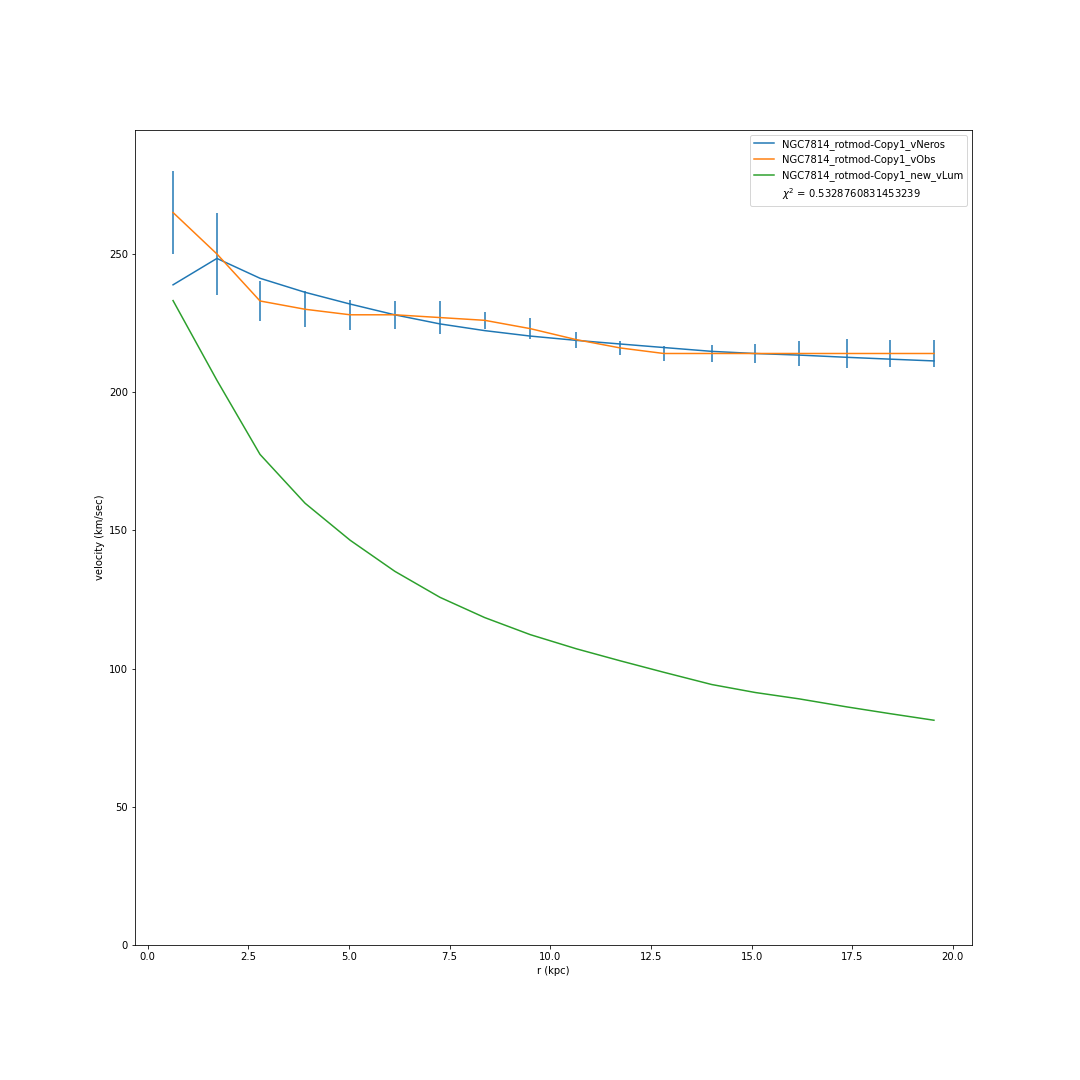
\includegraphics[width=.95\linewidth]{figures/NGC7814_rotmod-Copy1_XueSofue.png}
  \captionof{figure}{ NGC 7814, RCFM fit to SPARC\cite{2016Lelli}. Bulge dominated.}
  \label{fig:n7814sparc}
\end{minipage}%
\begin{minipage}{.5\textwidth}
  \centering
  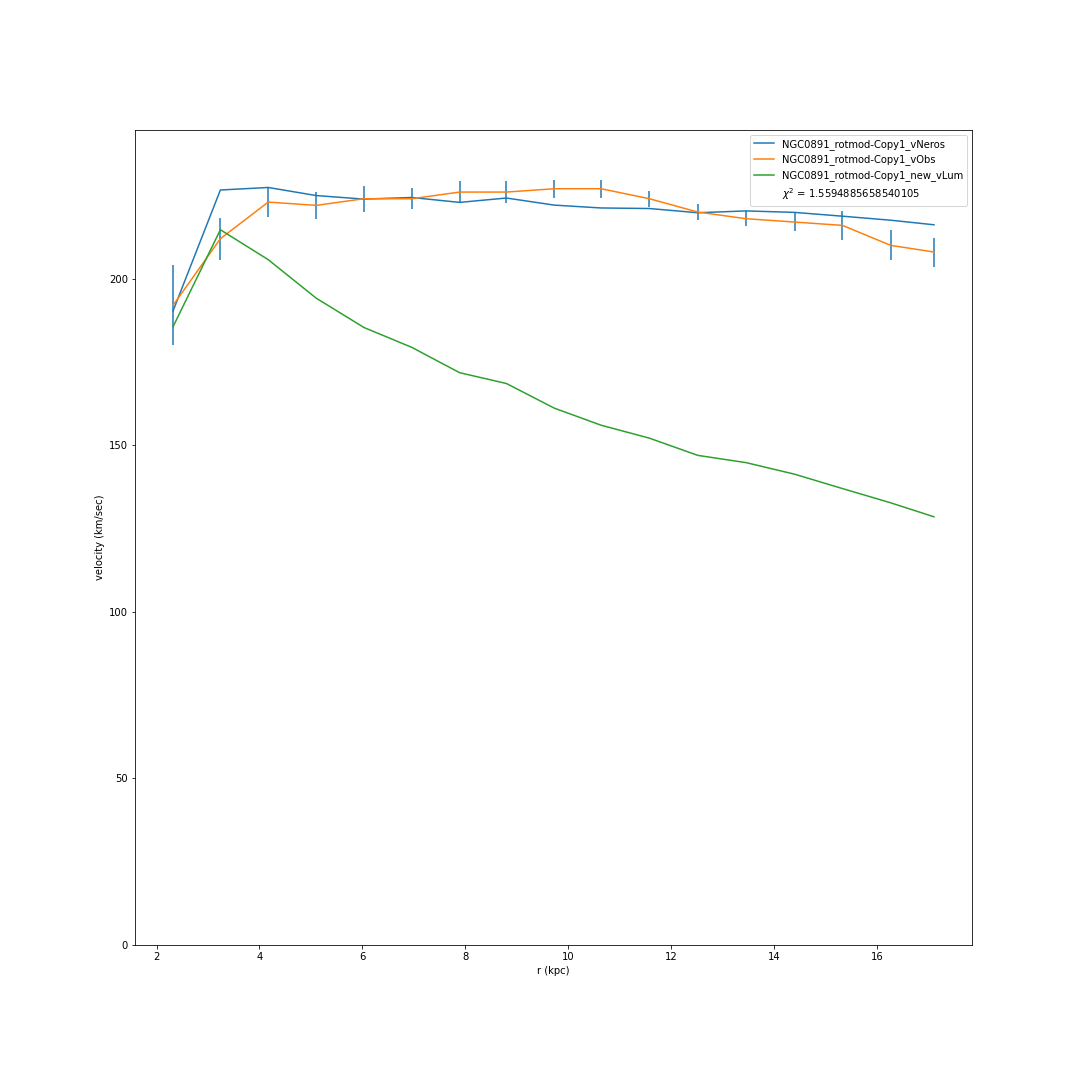
\includegraphics[width=.95\linewidth]{figures/NGC0891_rotmod-Copy1_XueSofue.png}
  \captionof{figure}{  NGC 891, RCFM fit to  SPARC\cite{2016Lelli},   Disk dominated }
  \label{fig:test1}
\end{minipage}
 \caption{Comparison of fits for NGC 7814 and NGC 891. Both edge-on galaxies with similar total light, but very different distributions of that light.     RCFM rotation curve fits (blue line), points with error bars are the rotation curve data, and the input baryonic mass models is  the green lines. {\color{blue}( (REMAKE with no orange line) } }\label{fitCompare7814_891}
\end{figure*}
 
 
 
 
  

\subsection{Free parameter functional form }\label{FreeCorrel}

  To test a guess at the functional form  for the  model's free parameter $\alpha$ based on photometric quantities, we first select a subset of galaxies with the most reliable distances and rotation curve data. 
  The selection  criteria are \cite{2016Lelli}. 
  \begin{enumerate}
      \item photometry interpreted with most reliable  distance methods    (tip of the red giant branch, and Cepheid variable stars,  with errors in distance on the order of $5\% - 10\%$), rejecting all other galaxies. \\
      \item  inclination angle on the sky  in the range  $[15^o, 80^o}$, rejecting galaxies with an inclination  greater than $80^o$ as impossible to constrain the surface brightness profile, and those at inclinations less than $15^o$ as being impossible to  report line of sight Doppler shifts accurately.
      \item  \citet{2016Lelli}   report a quality factor for each galaxy in the SPARC database, assigning  $Q=3$ to galaxies not suited to dynamical studies due to     asymmetries,  non-circular motions, and/or offsets between stars and gas. Galaxies with Q = 3 are rejected from our subset.
%not suited for detailed dynamical studies:
  \end{enumerate}
    By this process, we select a subset of 36 galaxies as reported in Table~\ref{tab:Tset}. 


 We then plot the  $\alpha$   parameter  space versus the ratio of  photometric quantities,  
  
\begin{equation}
    L_{total}/R_{eff}, 
\end{equation}
 
 for  $L_{total}$    the  total luminosity of the galaxy as measured  at a wavelength of $3.6 \mu m$,  assuming a solar
absolute magnitude of 3.24 at $3.6 \mu m$ \cite{oh2008high}, and the effective radius $R_{eff}$    the length encompassing half of the total luminosity \cite{2016Lelli}. 
 The resulting distribution    (Fig.~\ref{alpha2}) is  well fitted by the function 
 
   
  
\begin{equation}
    \alpha =  
    53.8 (L_{total}/R_{eff})^{-1.06}
       \label{FreeParamFix}
\end{equation}

at a confidence level of $83\%$.
{\color{blue}(UPDATED From Master RCFM 2.8.23)}
  
 \begin{figure}[h!]
%\scalebox{0.5}%
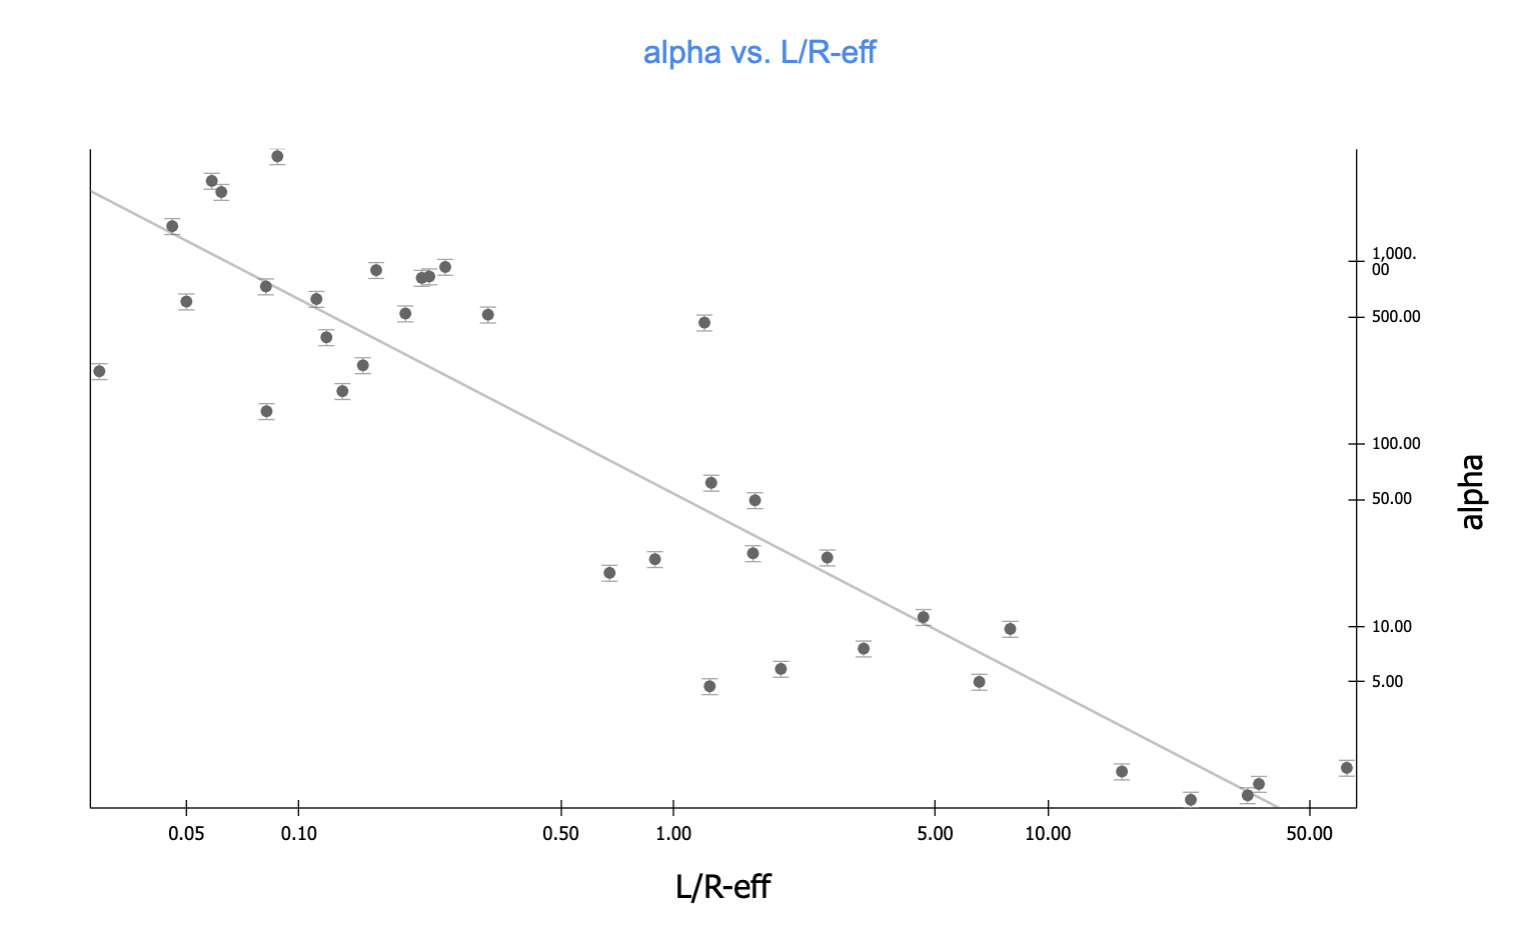
\includegraphics[width=\linewidth]{figures/alphavL_Reff2_8_23.png} 
\caption{ {\color{blue}(REMADE From Master RCFM 2.8.23), TSet updated. Need to make prettier.  Errors not real, but could use those reported on SPARC for LUM, and or Distance method - ask Rich or Amy??}.  Free-parameter functional interpretation in terms of  photometric parameters $L$ in units of $10^9$ solar  $L_\odot$ and $R_{eff}$ in kpc, using most reliable subset of galaxy data, see  Table~\ref{tab:Tset}.  }
\label{alpha2}
\end{figure}  
 
On inspection, the functional form in Eq.~\ref{FreeParamFix} might suggest a ratio with the same quantity for the Milky Way, as compared with   the RCFM mapping terms in $\kappa v_1 v_2$, which are all composed of ratios of the same quantity for the galaxy being observed with respect to the Milky Way(Reference Eq.~or Sec.). If we apply that reasoning to the relationship in Eq.~\ref{FreeParamFix}, then the same quantity for the Milky Way would be something of the form $42.9 =(L_{total}/R_{eff})_{mw} $. This is a very small subset of a high quality data set, but one can imagine with a large, statistically selected sample one might put  constrain from photometry  the mass of the Milky Way. 

{\color{blue}RICH, The phrasing sounds extremely strange/confusing to me: "We might assume that alpha is a ratio of the same quantity for the Milky Way ..." What is that supposed to mean? That it's a possible higher order fitting function? \color{teal} I'm not sure if it's a higher order fitting function or if we even want to try to constrain fits using this functional interpretation, but it does make our model a zero param model. Then again, we already have at least one fewer free parameters than MOND or Dark Matter, so it maybe doesn't matter. }
 
  %%NOTE:  Details on SPARC Mass models. 
  %%%%%%SPARC uses hybrid rotation curves on 56 galaxies, combining H-alpha  (inner) with HI (outer)
 %Face-on gals in SPARC."We assign a quality flag (Q) to each rotation curve using the following scheme: Q = 1 for galaxies with high-quality H I data or hybrid Hα/H I rotation curves (99 objects); Q = 2 for
%galaxies with minor asymmetries and/or H I data of lower
%quality (64 objects); Q = 3 for galaxies with major asymmetries, strong noncircular motions, and/or offsets between H I
%nd stellar distributions (12 objects). Galaxies with Q = 3 are%
%not suited for detailed dynamical studies: we build mass models
%for completeness but do not consider them in our analysis.
 


 



 
 \section{  Conclusions \label{sec:conclu}  }
 

The   rotation curve fitting model (RCFM) presented here      replaces dark matter with a series of  Lorentz-type transformations between     galaxy frames, subsuming the role of the dark matter with the Milky Way frame. 
Previous consideration of frame-dependency in this problem was obviated by Galilean subtraction of redshifts at the limit of the rotation curve data\cite{Wald}. The RCFM can be seen as a   relativistic extension of the MONDian idea of changing acceleration scales, without modifying Einstein's gravity, simply by transitioning the 
  MONDian idea of changing accelerations   to the concept of relative galaxy curvatures. 
The RCFM can be seen in this paper to reproduce the fitting successes of MOND,   on as  sample of   175  well studied galaxies\cite{2016Lelli},   to 
 reproduce physically reasonable mass-to-light ratios,    and to use only input parameters from photometry. 
However, interpreting the flat-rotation curve problem in this way  has multiple benefits as compared to MOND or dark matter models; as
  it  
   has   fewer free parameters (See Sec.~\ref{FreeCorrel}), 
  and   does not modify classical Einstein gravity or add particles to the standard model.
 




 The RCFM  requires a static choice of the Milky Way's  gravitational potential due to the baryon distribution to fit external galaxies. This means that this model is falsifiable with 
upcoming (the Legacy Survey of Space and Time (LSST)  \cite{Ivezić_2019})  and ongoing  surveys of millions of  stars in the Milky Way
 \cite{2022ApJS..259...35A,2010ApJ...716....1B,de_Blok_2010}. As can be seen in Fig.~\ref{fig:mwSofue}, the rotation curve of the Milky Way  is ambiguous  past  $8$kpc  in 
  the galactic disk. 

 
 
  The RCFM   as presented here   is a decidedly   heuristic treatment of the flat-rotation curve problem, simply replacing dark matter with a series of   Lorentz-type transformations between  weak gravitational frames. However, one would suppose if this approach proves to have merit that a more fundamental derivation may exist. 
  We do not address any of the other dark matter problems in cosmology in this paper. 
  
 %In example, the James Webb Space Telescope may have already falsified dark matter driven galaxy formation \cite{2022arXiv221014915H}.
   

  \section[]{Acknowledgments}
 This work is dedicated to Emmett Till, with respect and gratitude to the first nations peoples of;  the Coast Salish bands of Washington State, 
 the Cheyenne, Arapaho and Ute  Peoples of Colorado, and the Algonquian Peoples of Massachusetts. 
  The authors would like to thank    V.\,P.\,  Nair,   R.\, Walterbos, S.\ McGaugh,  A.\, Klypin, K. Bender, C. Beetle and     T.\, Boyer, M. Juric.   \\
  
 
% QUESTION FOR GROUP: how is our model predictive, more so than MOND, since we both do well on fitting galaxies. The Milky Way. We get a large enough sample of galaxies with certain distances and good photometry (SPARC) and run against a two MW. 
%ANSWER FOR GROUP: Our is twice as good on average chisquare value across the whole sample, has same number of free parameters as MOND, (our our MW and alpha) (MOND's are acceleration scale and distance), and we about the same for the mass-to-light ratios as compared to the populations synthesis models. The key science difference is our reproduces rotation curves of very well studied galaxies with super reliable distance indicator (Cepheid variable stars) at the correct distance and MOND has to put them at distances that are up to 2sigma different. ALso, MOND requires modication of Einsteins' gravity, which is super well tested at least locally, and our doesnt'. So, for my money, we win. SNC.

%%%%%%%
 

\begin{figure*}
\centering
\begin{minipage}{.5\textwidth}
  \centering
  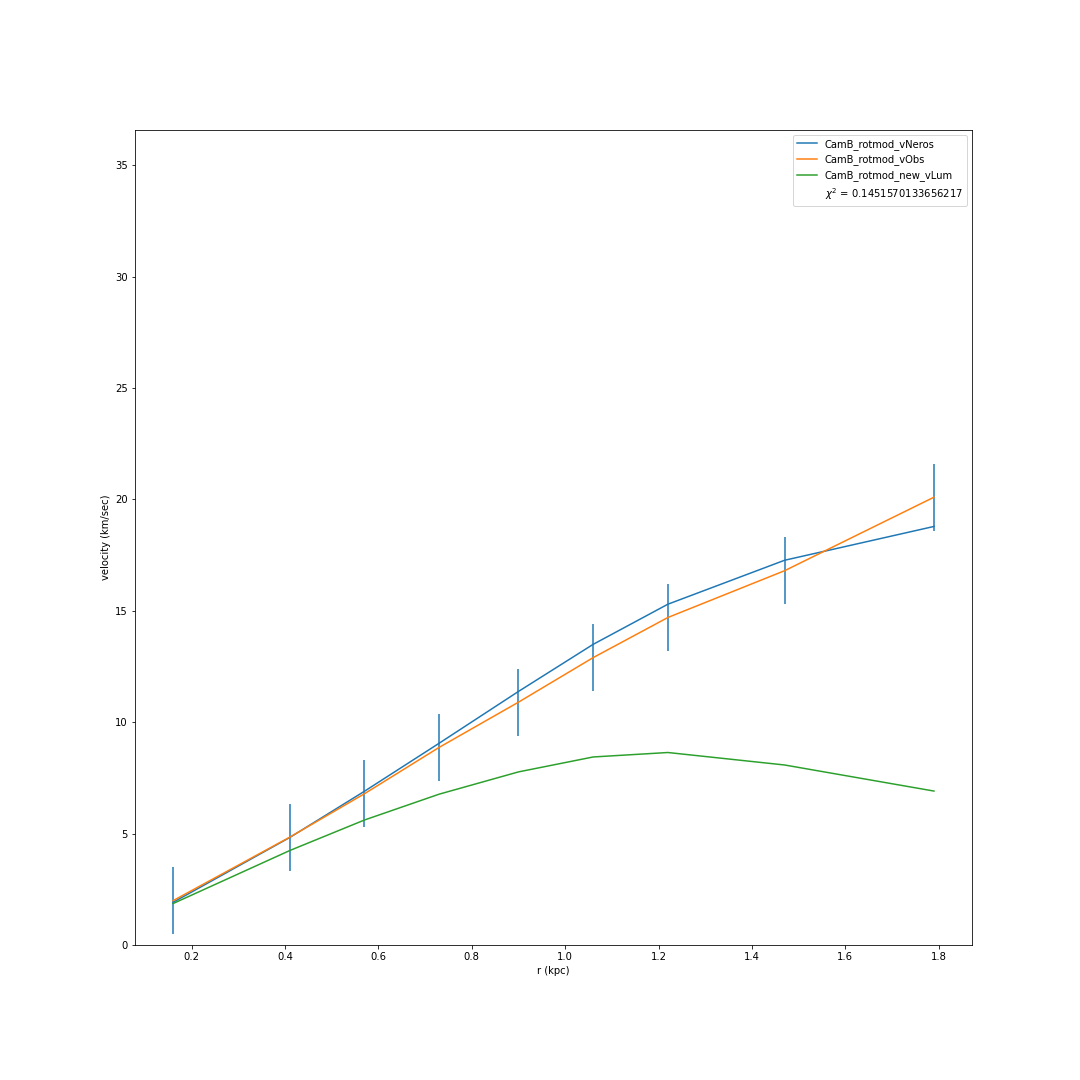
\includegraphics[width=.95\linewidth]{figures/CamB_rotmod_XueSofue.png}
  \captionof{figure}{CamB : SPARC\cite{2016Lelli}}
  \label{fig:test1}
\end{minipage}%
\begin{minipage}{.5\textwidth}
  \centering
  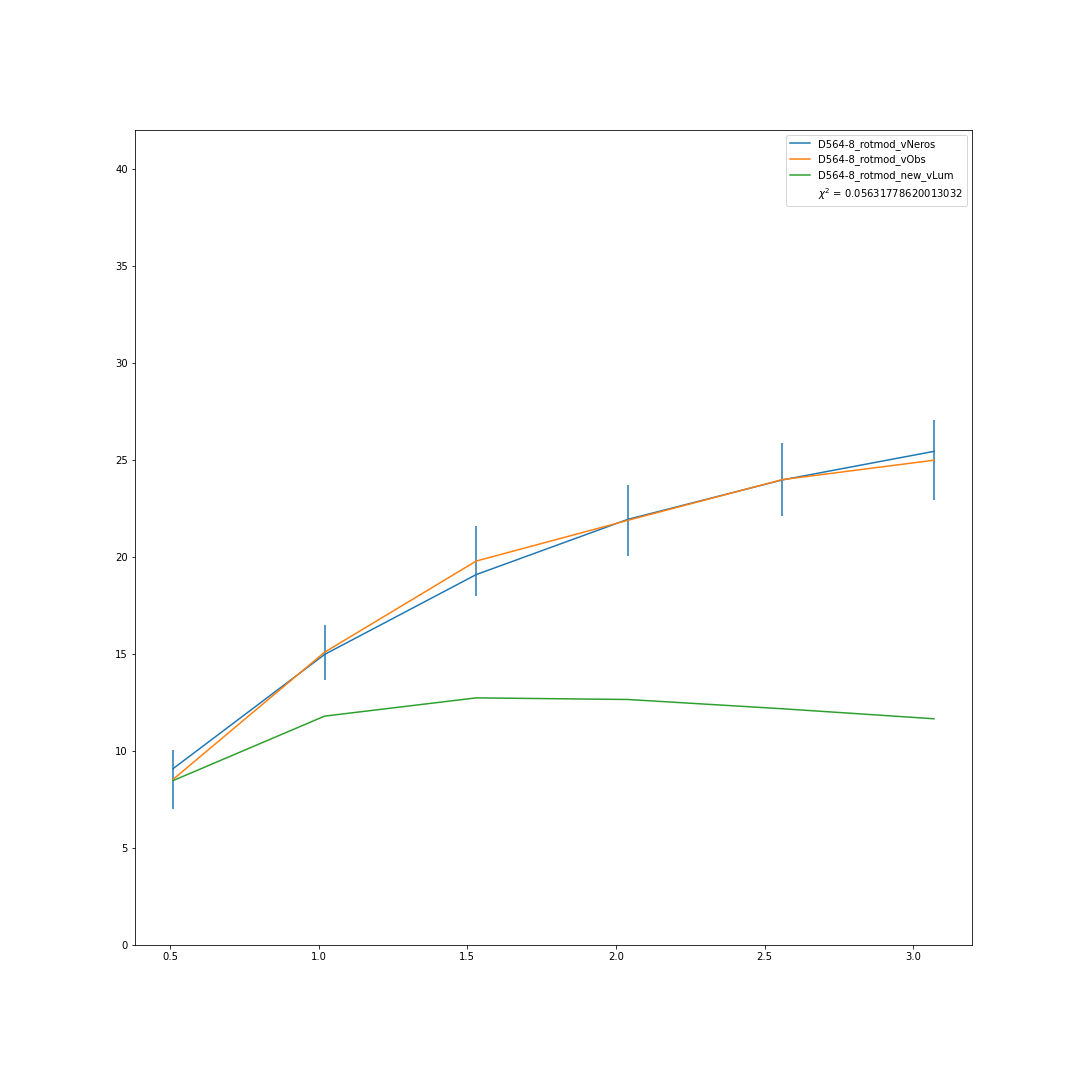
\includegraphics[width=.95\linewidth]{figures/D564-8_rotmod_XueSofue.png}
  \captionof{figure}{D564-8 : SPARC\cite{2016Lelli}}
  \label{fig:test2}
\end{minipage}
\begin{minipage}{.5\textwidth}
  \centering
  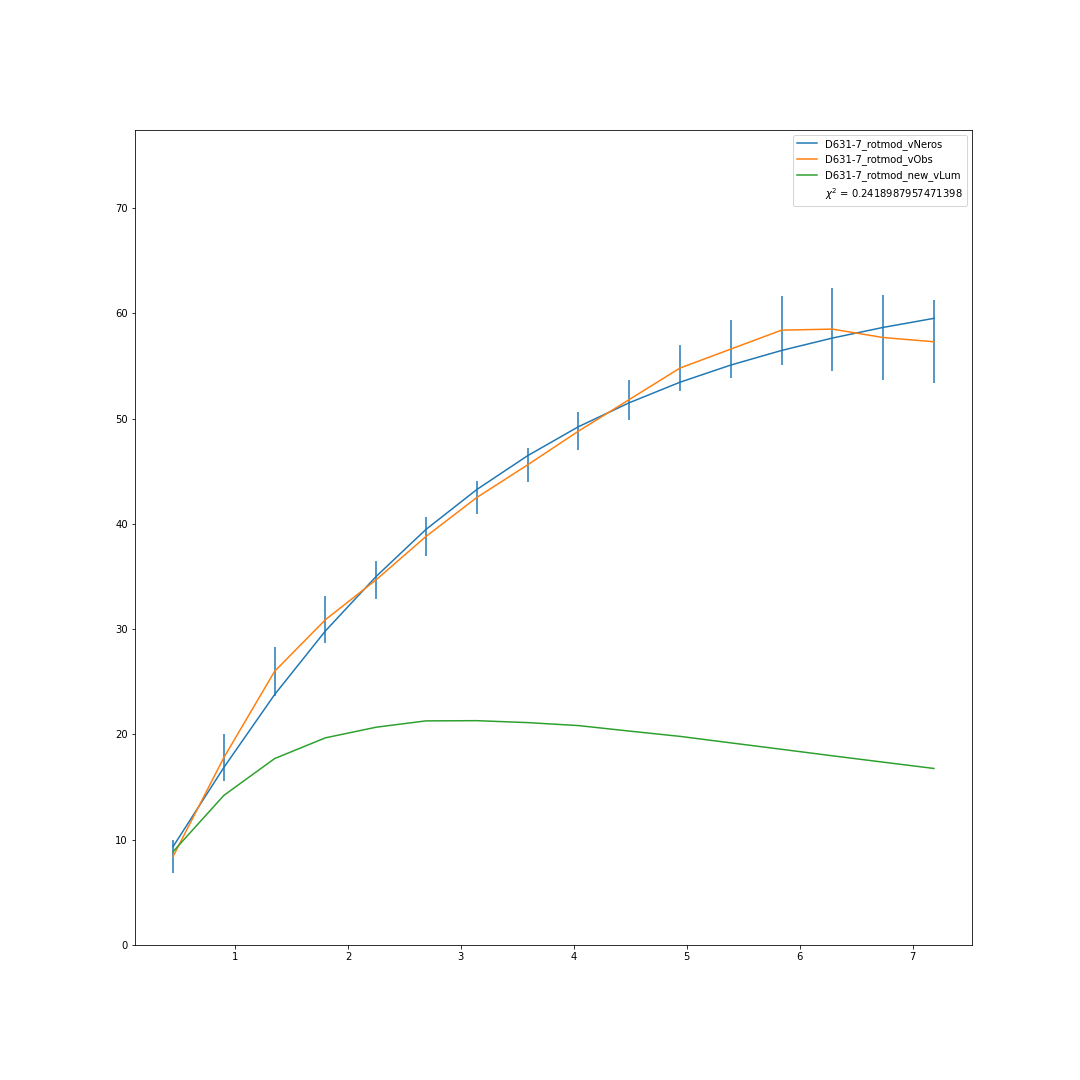
\includegraphics[width=.95\linewidth]{figures/D631-7_rotmod_XueSofue.png}
  \captionof{figure}{D631-7  SPARC\cite{2016Lelli}}
  \label{fig:test1}
\end{minipage}%
\begin{minipage}{.5\textwidth}
  \centering
  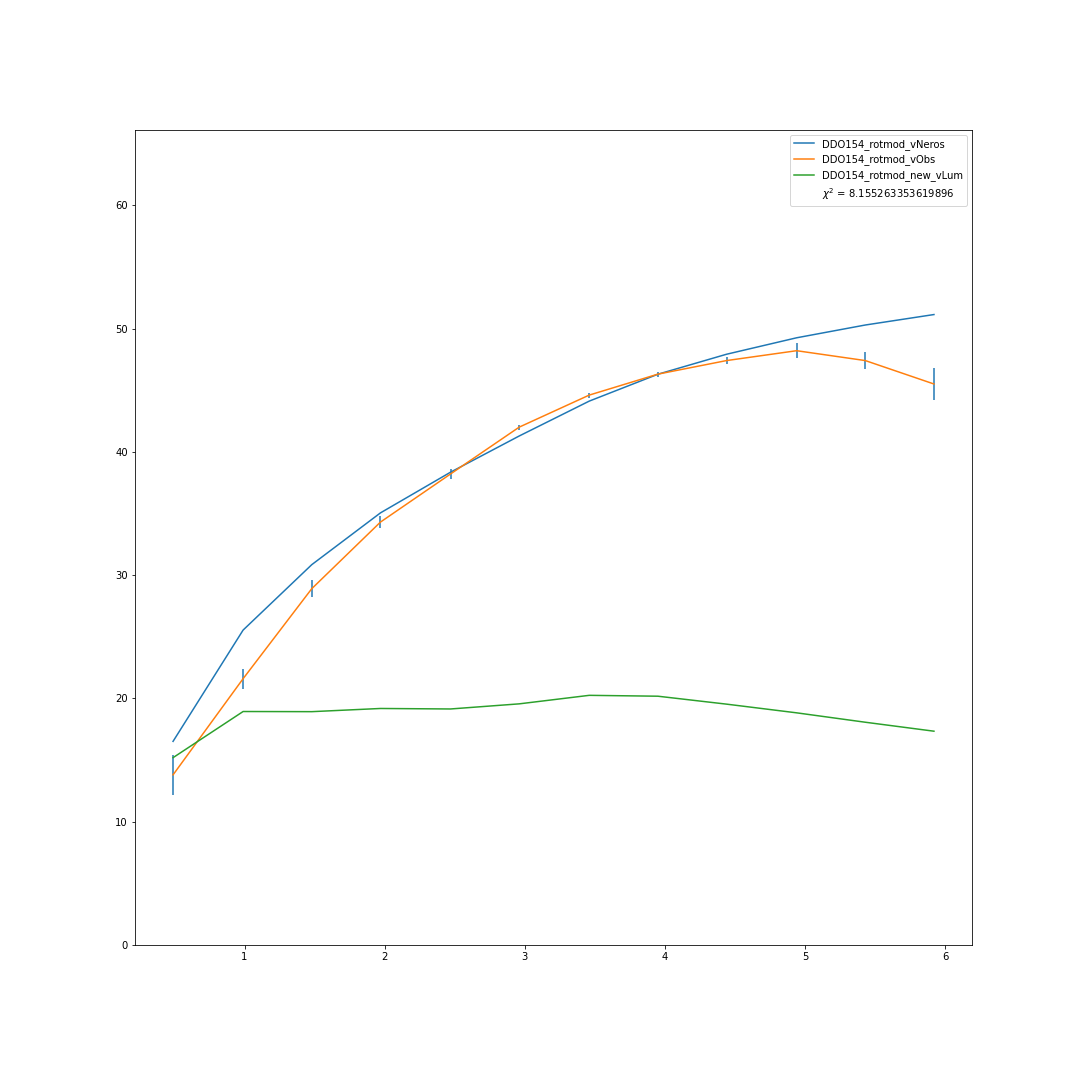
\includegraphics[width=.95\linewidth]{figures/DDO154_rotmod_XueSofue.png}
  \captionof{figure}{DD00154 : SPARC\cite{2016Lelli}}
  \label{fig:test1}
\end{minipage}
 \caption{Examples of range of gas dominated, dwarf galaxies, their RCFM rotation curve fits (blue line), points with error bars are the rotation curve data, and the input baryonic mass models is  the green lines. (MARCUS PAZ : NOTE: remove orange lines, fit through data distracts from our fit)  }
\end{figure*}
 
            
\begin{figure*}
\centering
\begin{minipage}{.5\textwidth}
  \centering
  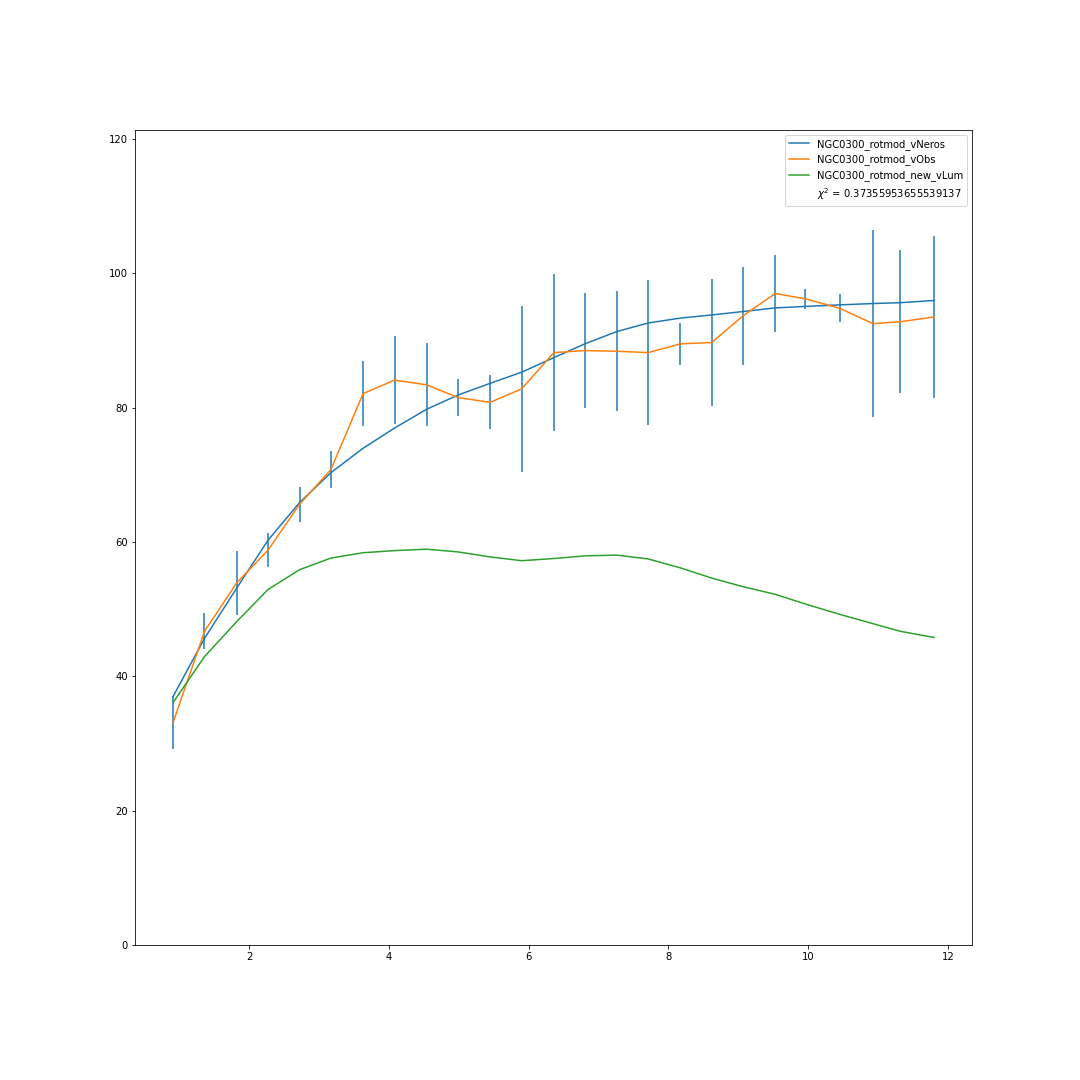
\includegraphics[width=.95\linewidth]{figures/NGC0300_rotmod_XueSofue.png}
  \captionof{figure}{ NGC0300 SPARC\cite{2016Lelli}}
  \label{fig:test1}
\end{minipage}%
\begin{minipage}{.5\textwidth}
  \centering
  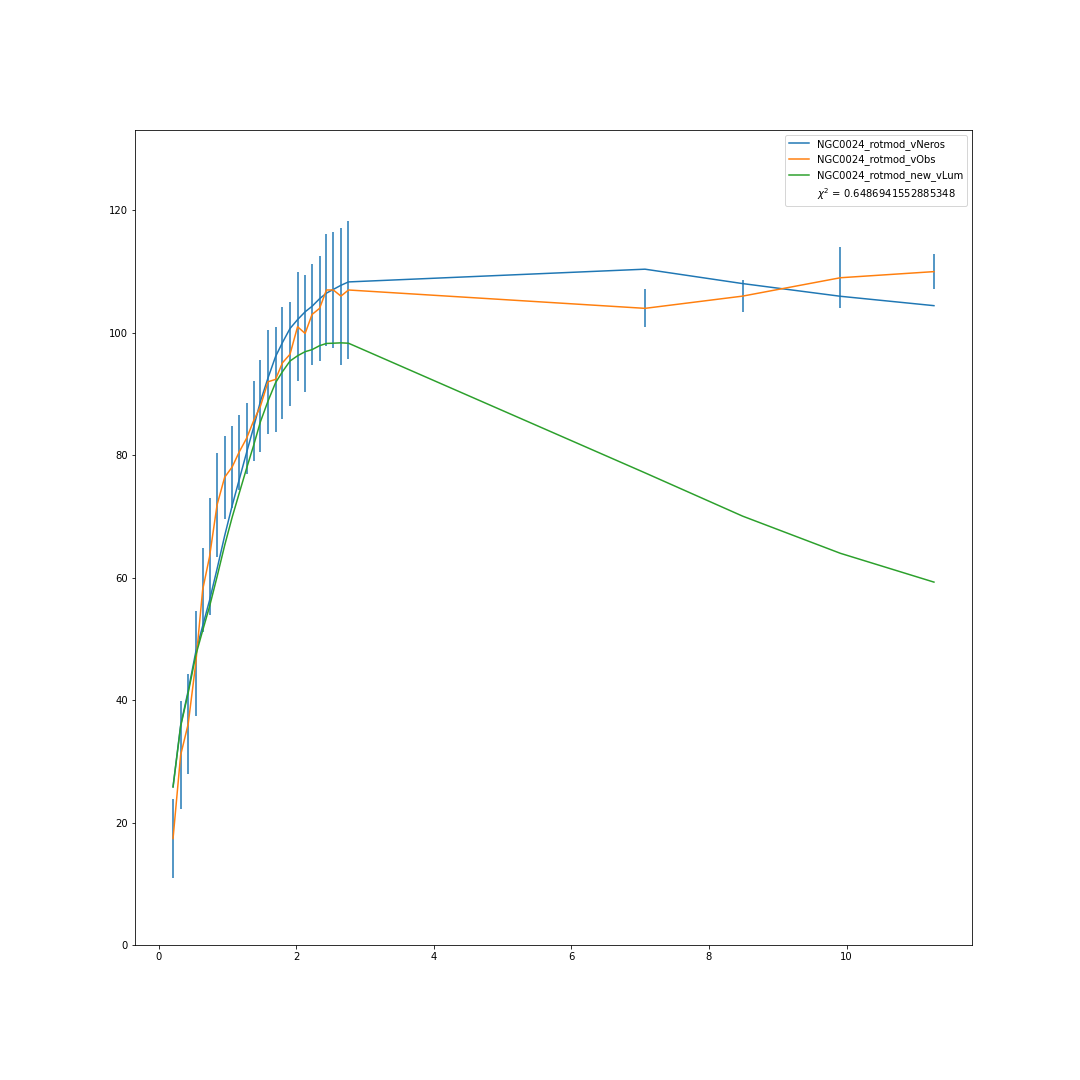
\includegraphics[width=.95\linewidth]{figures/NGC0024_rotmod_XueSofue.png}
  \captionof{figure}{ NGC0024 SPARC\cite{2016Lelli}}
  \label{fig:test2}
\end{minipage}
\begin{minipage}{.5\textwidth}
  \centering
  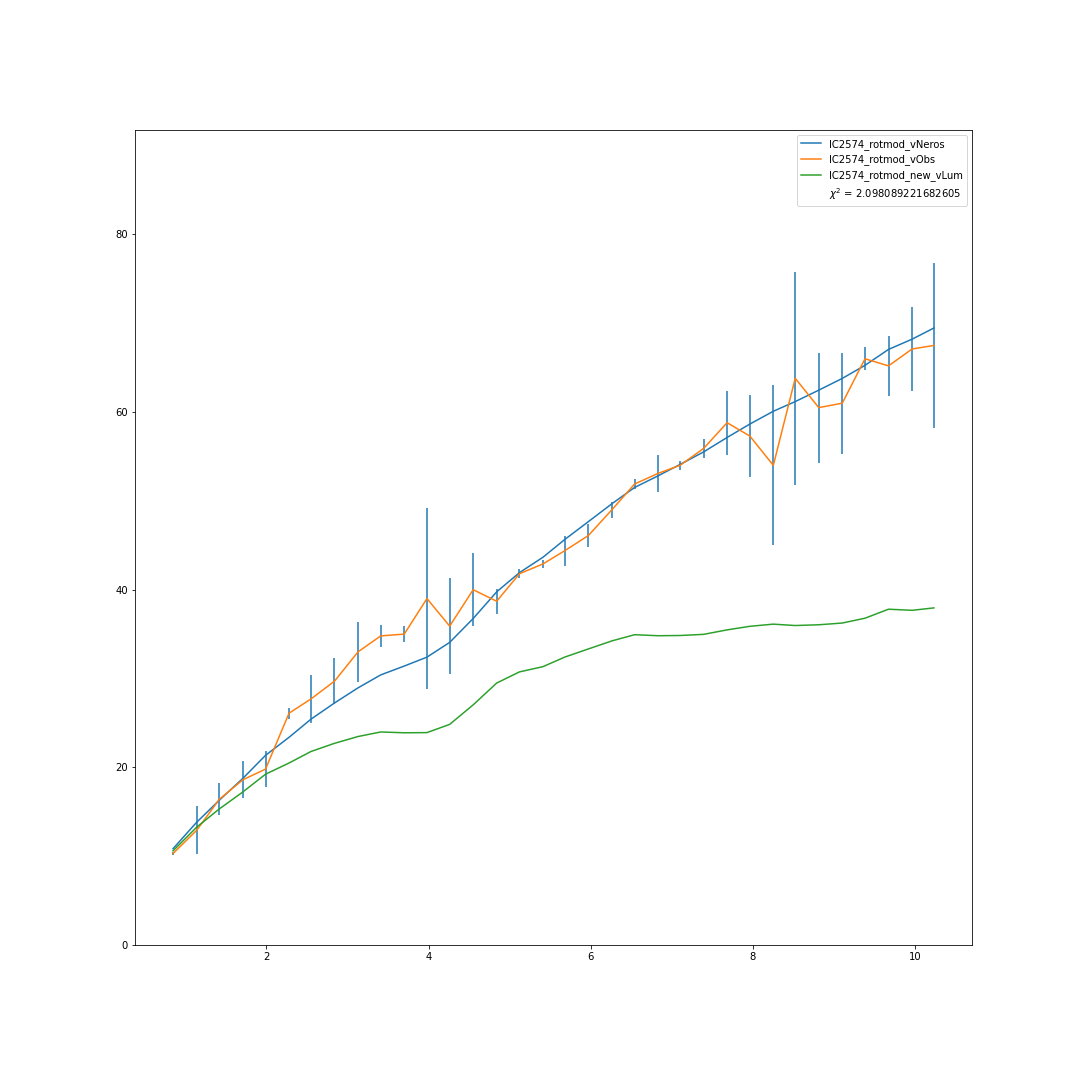
\includegraphics[width=.95\linewidth]{figures/IC2574_rotmod_XueSofue.png}
  \captionof{figure}{ IC2574  SPARC\cite{2016Lelli}}
  \label{fig:test1}
\end{minipage}%
\begin{minipage}{.5\textwidth}
  \centering
  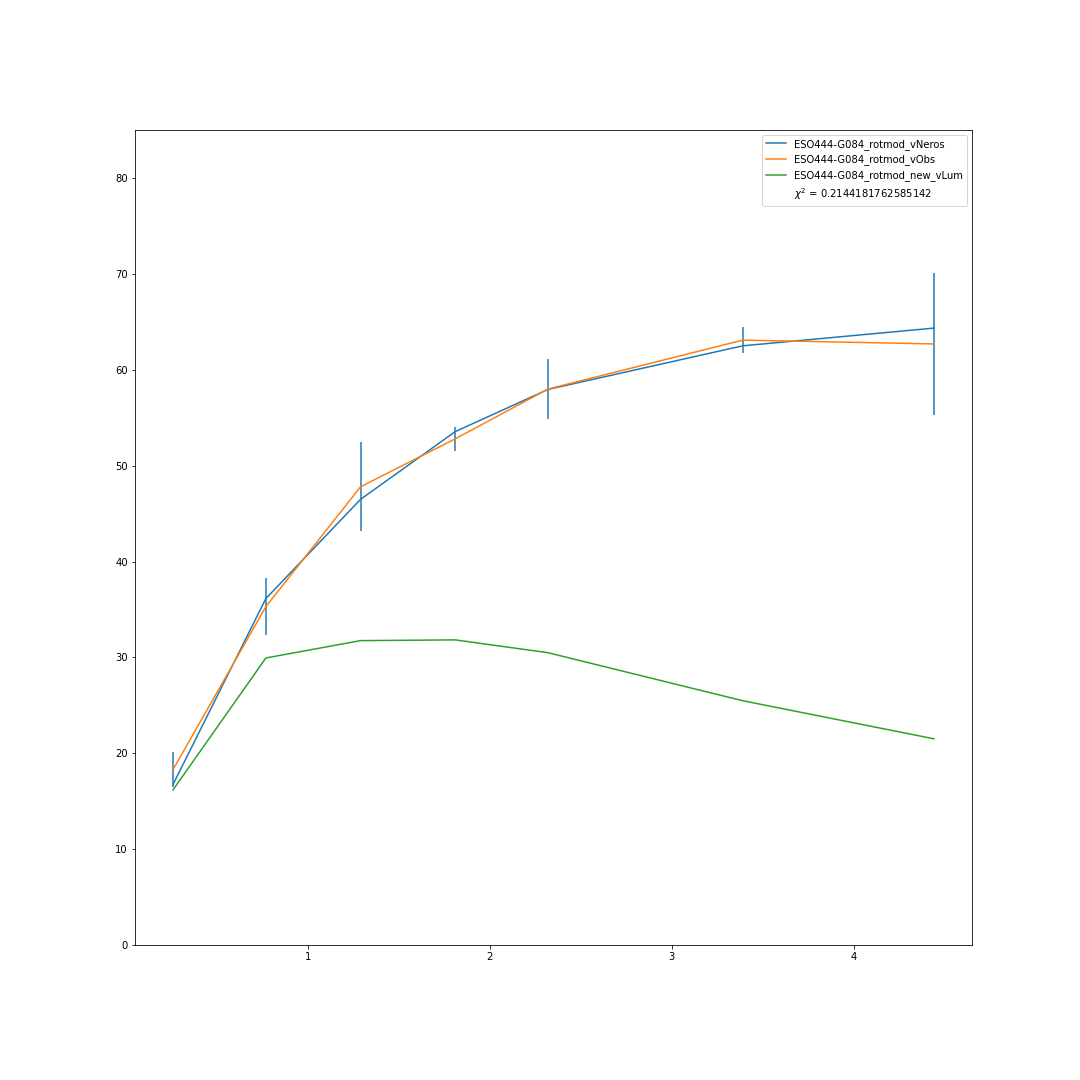
\includegraphics[width=.95\linewidth]{figures/ESO444-G084_rotmod_XueSofue.png}
  \captionof{figure}{ ESO444-G084 SPARC\cite{2016Lelli}}
  \label{fig:test1}
\end{minipage}
 \caption{Example  RCFM rotation curve fits (blue line), points with error bars are the rotation curve data, and the input baryonic mass models is  the green lines. (MARCUS PAZ : NOTE: remove orange lines, fit through data distracts from our fit)  }
\end{figure*}
 %%%%%%%
    %%%%%%%
      %%%%%%%
        %%%%%%%
          %%%%%%%
            %%%%%%%
\begin{figure*}
\centering
\begin{minipage}{.5\textwidth}
  \centering
  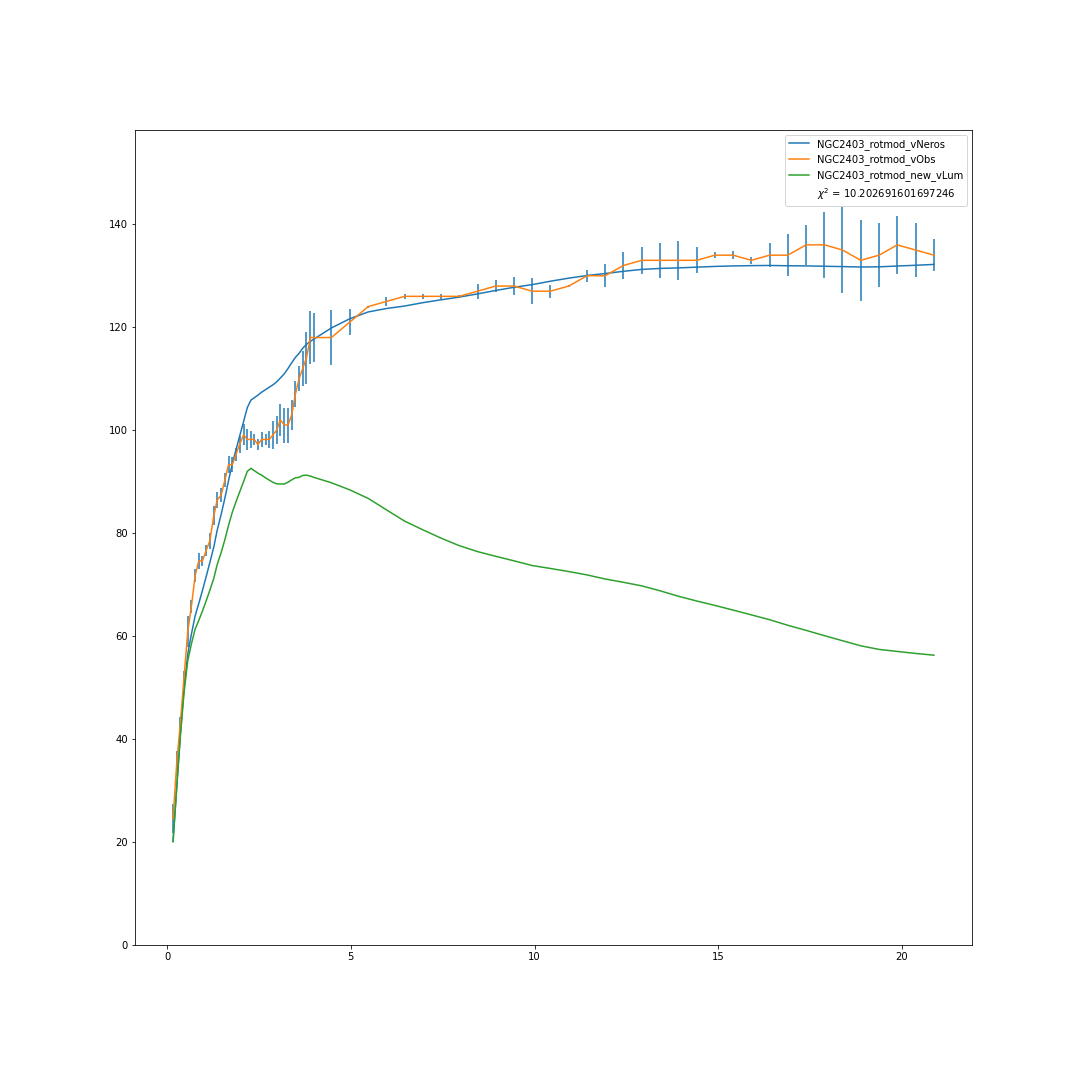
\includegraphics[width=.95\linewidth]{figures/NGC2403_rotmod_XueSofue.png}
  \captionof{figure}{ NGC2403 SPARC\cite{2016Lelli}}
  \label{fig:test1}
\end{minipage}%
\begin{minipage}{.5\textwidth}
  \centering
  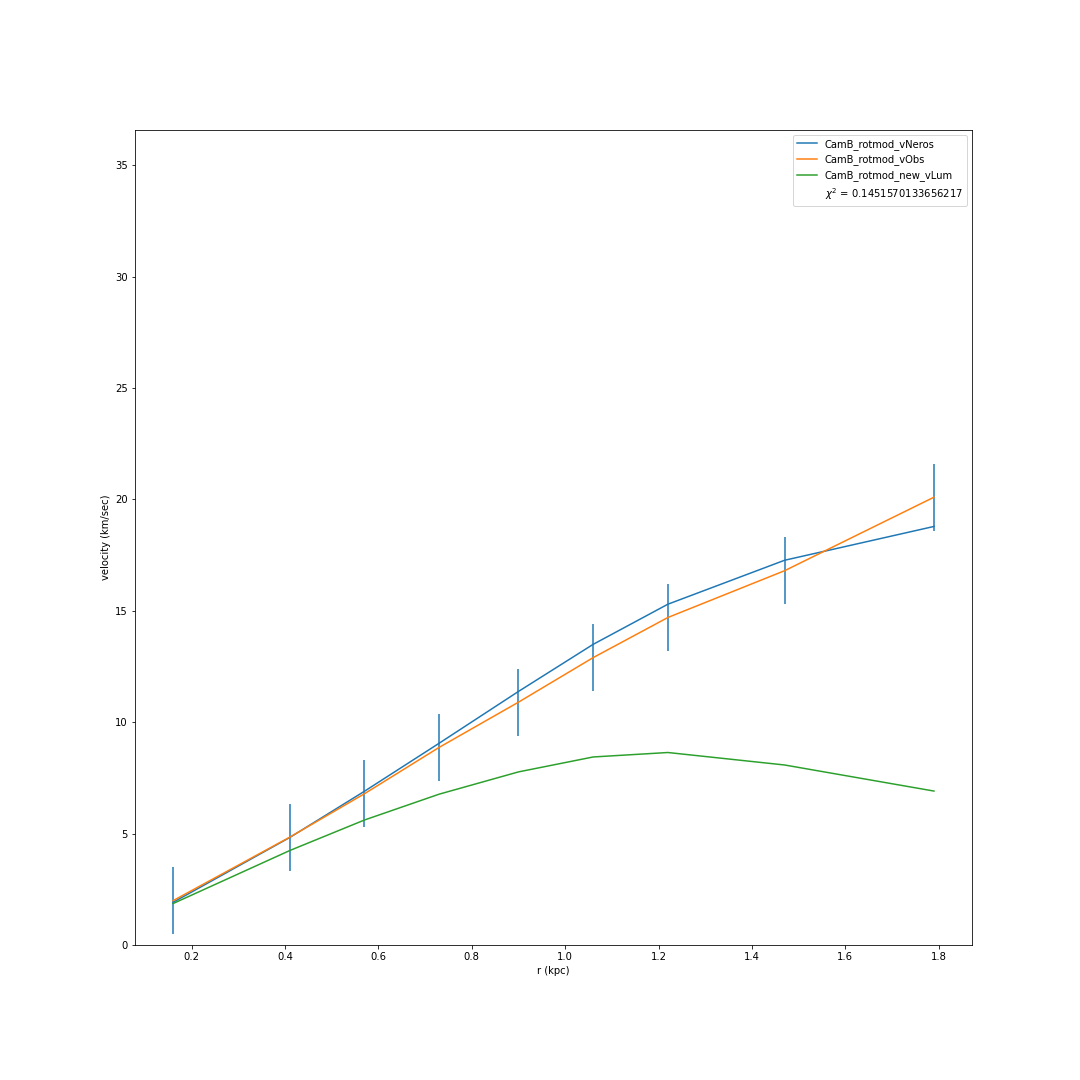
\includegraphics[width=.95\linewidth]{figures/CamB_rotmod_XueSofue.png}
  \captionof{figure}{ CamB  from SPARC\cite{2016Lelli}}
  \label{fig:test2}
\end{minipage}
\begin{minipage}{.5\textwidth}
  \centering
  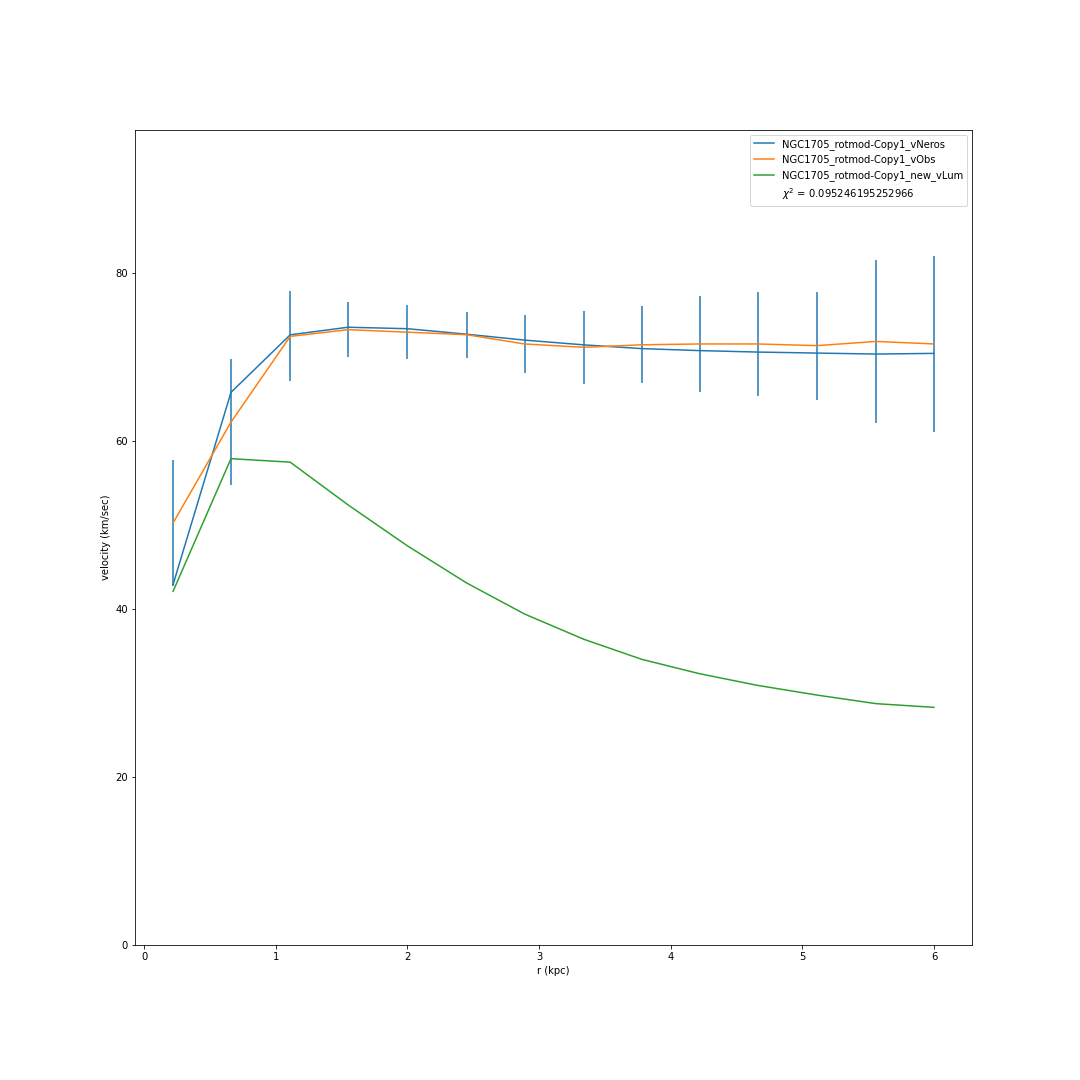
\includegraphics[width=.95\linewidth]{figures/NGC1705_rotmodXueSofue.png}
  \captionof{figure}{ NGC1705  SPARC\cite{2016Lelli}}
  \label{fig:test1}
\end{minipage}
 \caption{Example  RCFM rotation curve fits (blue), rotation curve data points with error bars (blue), and   luminous  mass models (green line). {\color{teal}NOTE: remove orange lines through data distracts, and change color of    RCFM fit to be different than data.)}  }
\end{figure*}
            %%%%%%%  %%%%%%%
  %%%%%%%   %%%%%%%  %%%%%%%
  %%%%%%%  %%%%%%%  %%%%%%%
  %%%%%%%
%%%%%%%
 %%%%%%%
 %%%%%%%
%%%%%%%
 %%%%%%%
%%%%%%%
%%%%%%%
%%%%%%%
 
 
%%%%%%%
\begin{figure} 
\centering
\begin{minipage}{0.5\textwidth}
%\centering
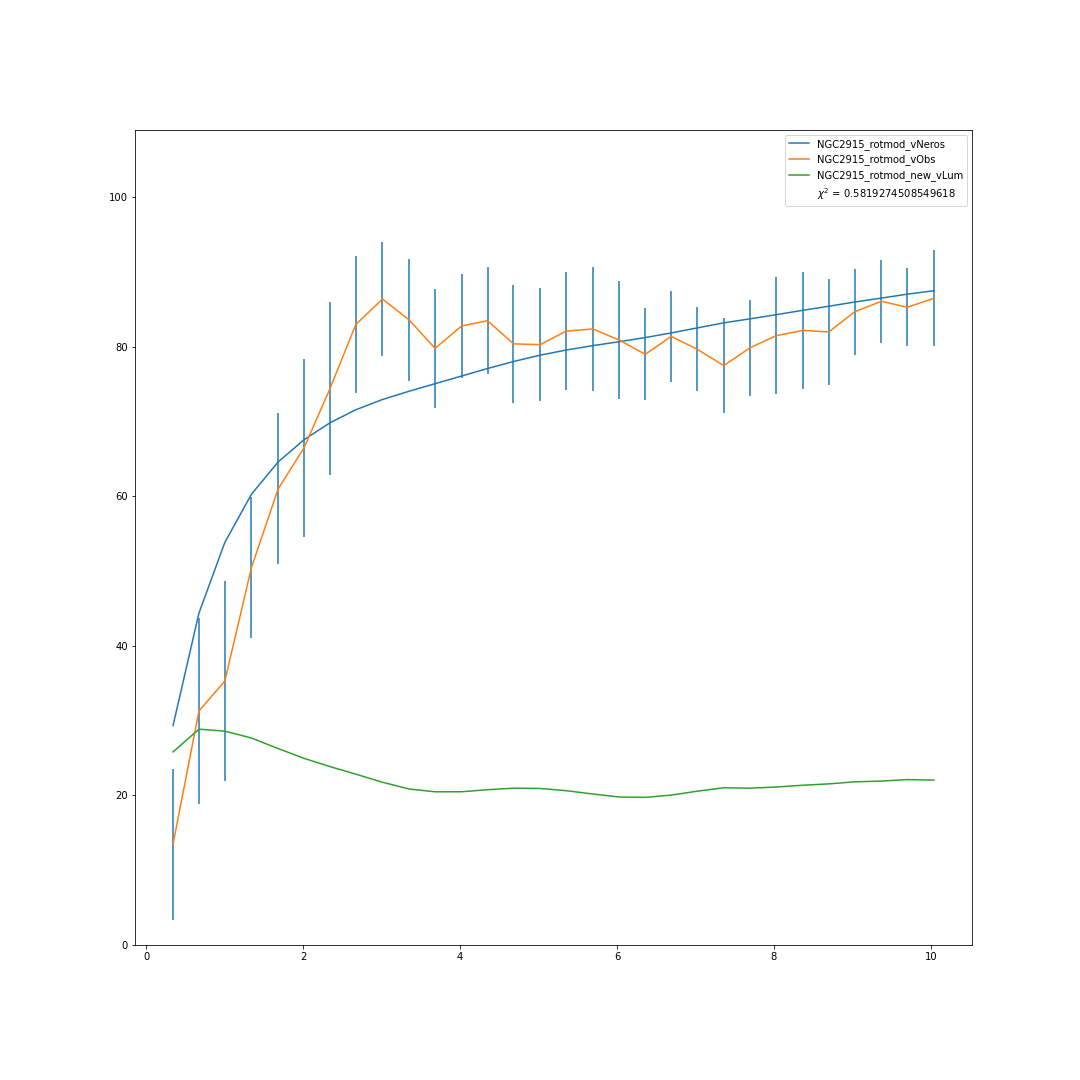
\includegraphics[width=0.95\linewidth]{figures/NGC2915_rotmod_XueSofue.png}
\caption{NGC 2915 SPARC\cite{2016Lelli}}
\label{fig:2915}
\end{minipage}
\begin{minipage}{0.5\textwidth}
%\centering
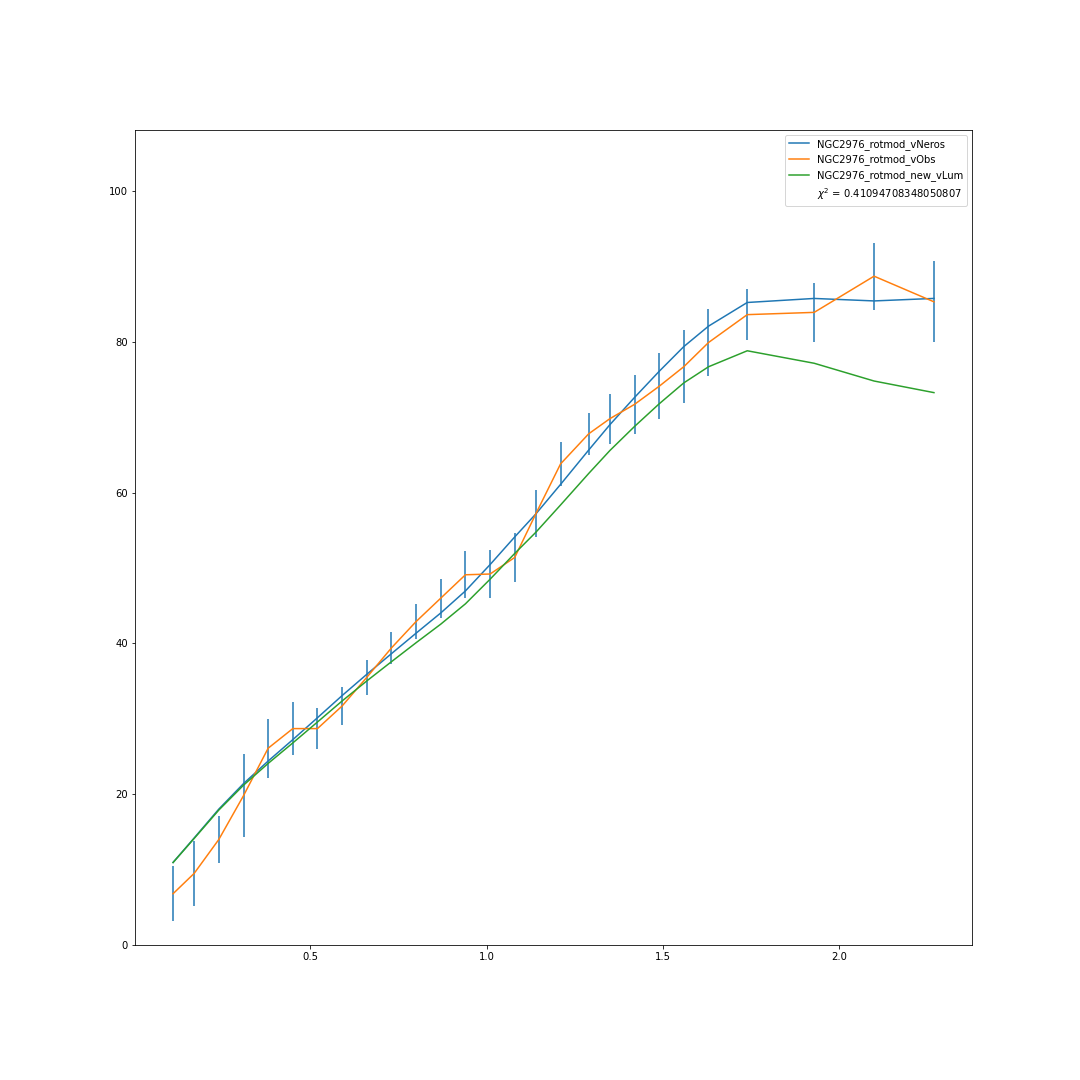
\includegraphics[width=0.95\linewidth]{figures/NGC2976_rotmod_XueSofue.png}
\caption{NGC 2976}
\label{fig:2976}
\end{minipage}
\end{figure}
%%%%%%%
%%%%%%%%
%%%%%%
%%%%%%%
%%%%%%
  
 

% Subset of galaxies to constrain RCFM free parameter }  }    \\
  \begin{table*}[]
      \centering
      \begin{tabular}{|c|c|c|c|c|c|}
      \hline \hline
\rowcolor[HTML]{CCCCCC} 
\textbf{Galaxy Name} & Hubble Type(1)& 	Distance (Mpc)&Mean Error on D (Mpc)& 	Distance Method (2)& 	Inc (deg)(3)\\
    \hline \hline\\
CamB&   	10&    3.36&  	0.26&   2&  65\\
D564-8& 	10& 	8.79& 	0.28& 	2& 	63\\
D631-7& 	10& 	7.72& 	0.18& 	2& 	59\\
DDO154& 	10& 	4.04& 	0.2& 	2& 	64\\
DDO168& 	10& 	4.25& 	0.21& 	2& 	63\\
ESO444-G084& 10& 	4.83& 	0.48& 	2& 	32\\
IC2574& 	9& 	3.91& 	0.2&    	2& 	75\\
NGC0024& 	5& 	7.3& 	0.36&   	2& 	64\\
NGC0055& 	9& 	2.11& 	0.11&   	2& 	77\\
NGC0247& 	7& 	3.7& 	0.19&   	2& 	74\\
NGC0300& 	7& 	2.08& 	0.1&    	2& 	42\\
NGC2403& 	6& 	3.16& 	0.16&   	2& 	63\\
NGC2683& 	3& 	9.81& 	0.49&   	2& 	80\\
NGC2841& 	3& 	14.1& 	1.4&    	3& 	76\\
NGC2915& 	11& 	4.06& 	0.2& 	2& 	56\\
NGC2976& 	5& 	3.58& 	0.18&   	2& 	61\\
NGC3109& 	9& 	1.33& 	0.07&   	2& 	70\\
NGC3198& 	5& 	13.8& 	1.4&    	3& 	73\\
NGC3741& 	10& 	3.21& 	0.17& 	2& 	70\\
NGC4068& 	10& 	4.37& 	0.22& 	2& 	44\\
NGC4214& 	10& 	2.87& 	0.14& 	2& 	15\\
NGC5055& 	4& 	9.9& 	0.3&    	2& 	55\\
NGC6503& 	6& 	6.26& 	0.31&   	2& 	74\\
NGC6789& 	11& 	3.52& 	0.18& 	2& 	43\\
NGC6946& 	6& 	5.52& 	1.66&   	2& 	38\\
NGC7331& 	3& 	14.7& 	1.5&    	3& 	75\\
NGC7793& 	7& 	3.61& 	0.18&   	2& 	47\\\
UGC04483& 	10& 	3.34& 	0.31& 	2& 	58\\
UGC07232& 	10& 	2.83& 	0.17& 	2& 	59\\
UGC07524& 	9& 	4.74& 	0.24& 	    2& 	46\\
UGC07559& 	10& 	4.97& 	0.25& 	2& 	61\\
UGC07577& 	10& 	2.59& 	0.13& 	2& 	63\\
UGC07866& 	10& 	4.57& 	0.23& 	2& 	44\\
UGC08490& 	9& 	4.65& 	0.53&   	2& 	50\\
UGC08837& 	10& 	7.21& 	0.36& 	2& 	80\\
UGCA442& 	9& 	4.35& 	0.22& 	    2& 	64\\
UGCA444& 	10& 	0.98& 	0.05& 	2& 	78\\
    \hline \hline           
      \end{tabular}
      \caption{{\color{blue}(UPDATED TSet on Master RCFM 2.8.23)}.
      Subset of galaxies to constrain RCFM free parameter $\alpha$.  
      (1) Hubble type 
of: 0 = S0, 1 = Sa, 2 = Sab,
3 = Sb, 4 = Sbc, 5 = Sc, 6 = Scd, 7 = Sd, 8 = Sdm,
9 = Sm, 10 = Im, 11 = BCD. 
(2) Distance method:  
2 = tip of the red giant branch, 3 = Cepheids.  (3) Inclination on the sky. All table information from \citet{2016Lelli}. } \label{tab:Tset}
  \end{table*}
 
 
 
 
\begingroup  
\setlength\extrarowheight{2pt}
\small
\setlength\LTcapwidth\textwidth
\begin{longtable*}{|c|c|c|c|c|c|c|c| }

\caption{\textbf{{\color{blue}(UPDATE From Master -  REMAKE TABLE }.
Comparison of Fit Results from RAR and RCFM  } } \label{table:M2Light} \\
\hline
\rowcolor[HTML]{CCCCCC} 
\textbf{Galaxy name} 
& \textbf{log (L{[}3.6{]})($L_\odot $)} 
& RAR $\gamma_{disk}$  
& RAR $\gamma_{bulge}$ 
&  RAR $\chi^2$ ave=4.22 
&\textbf{RCFM}$\chi^2$ ave=1.8
&\textbf{RCFM} $\gamma_{disk}$
&\textbf{RCFM} $\gamma_{bulge}$

\\
\hline
\endfirsthead 

\multicolumn{8}{@{}l}{\tablename~\thetable, cont'd.} \\[0.5ex]
\hline
\rowcolor[HTML]{CCCCCC} 
\textbf{Galaxy name} 
& \textbf{ (L{[}3.6{]})($10^9 L_\odot $)} 
& RAR $\gamma_{disk}$  
& RAR $\gamma_{bulge}$ 
&  RAR $\chi^2$ ave=4.22 
&\textbf{RCFM}$\chi^2$ ave=1.8
&\textbf{RCFM} $\gamma_{disk}$
&\textbf{RCFM} $\gamma_{bulge}$
 \\ \hline
\endhead 

\multicolumn{5}{r@{}}{\em Cont'd on following page}\\
\endfoot

\endlastfoot

%% Body of table
CamB                 & 7.88                      & 0.34 ± 0.08           & …                      & 5.758                                                        & 0.145                                                          & 1.43E-05                                                              & …                                                             \\
\rowcolor[HTML]{F3F3F3} 
D512-2               & 8.51                      & 0.48 ± 0.12           & …                      & 0.37                                                         & 0.052                                                       & 1.48                                                           & …                                                             \\
\rowcolor[HTML]{F3F3F3} 
D564-8               & 7.52                      & 0.40 ± 0.09           & …                      & 3.16                                                         & 0.056                                                          & 1.22                                                           & …                                                             \\
\rowcolor[HTML]{F3F3F3} 
D631-7               & 8.29                      & 0.20 ± 0.04           & …                      & 15.872                                                       & 0.242                                                         & 0.28                                                           & …                                                             \\
\rowcolor[HTML]{F3F3F3} 
DDO064               & 8.2                       & 0.48 ± 0.11           & …                      & 0.334                                                        & 0.357                                                         & 1.58                                                           & …                                                             \\
\rowcolor[HTML]{F3F3F3} 
DDO154               & 7.72                      & 0.19 ± 0.03           & …                      & 3.482                                                        & 8.155                                                            & 1.20                                                          & …                                                             \\
\rowcolor[HTML]{F3F3F3} 
DDO161               & 8.74                      & 0.23 ± 0.04           & …                      & 1.468                                                        & 0.585                                                         & 0.98                                                           & …                                                             \\
\rowcolor[HTML]{F3F3F3} 
DDO168               & 8.28                      & 0.46 ± 0.11           & …                      & 19.714                                                       & 3.087                                                           & 0.79                                                          & …                                                             \\
\rowcolor[HTML]{F3F3F3} 
DDO170               & 8.73                      & 0.79 ± 0.15           & …                      & 4.917                                                        & 2.006                                                            & 1.84                                                           & …                                                             \\
\rowcolor[HTML]{F3F3F3} 
ESO079-G014          & 10.71                     & 0.50 ± 0.09           & …                      & 4.334                                                        & 3.081                                                          & 1.09                                                            & …                                                             \\
\rowcolor[HTML]{F3F3F3} 
ESO116-G012          & 9.63                      & 0.35 ± 0.04           & …                      & 2.444                                                        & 0.842                                                        & 1.04                                                          & …                                                             \\
\rowcolor[HTML]{F3F3F3} 
ESO444-G084          & 7.85                      & 0.42 ± 0.09           & …                      & 3.253                                                        & 0.214                                                          & 1.87                                                           & …                                                             \\
\rowcolor[HTML]{F3F3F3} 
ESO563-G021          & 11.49                     & 0.43 ± 0.04           & …                      & 28.836                                                       & 14.570                                                          & 0.99                                                          & …                                                             \\
\rowcolor[HTML]{F3F3F3} 
F561-1               & 9.61                      & 0.52 ± 0.13           & …                      & 1.564                                                        & 0.525                                                          & 0.96                                                          & …                                                             \\
\rowcolor[HTML]{F3F3F3} 
F563-1               & 9.28                      & 0.56 ± 0.12           & …                      & 1.499                                                        & 0.788                                                         & 2.07                                                           & …                                                             \\
\rowcolor[HTML]{F3F3F3} 
F563-V1              & 9.19                      & 0.48 ± 0.12           & …                      & 0.875                                                        & 0.143                                                         & 0.99                                                           & …                                                             \\
\rowcolor[HTML]{F3F3F3} 
F563-V2              & 9.48                      & 0.59 ± 0.14           & …                      & 0.991                                                        & 0.079                                                       & 2.20                                                           & …                                                             \\
\rowcolor[HTML]{F3F3F3} 
F565-V2              & 8.75                      & 0.50 ± 0.12           & …                      & 0.474                                                        & 0.181                                                        & 2.23                                                           & …                                                             \\
\rowcolor[HTML]{F3F3F3} 
F567-2               & 9.33                      & 0.56 ± 0.13           & …                      & 2.204                                                        & 0.200                                                       & 1.31                                                           & …                                                             \\
\rowcolor[HTML]{F3F3F3} 
F568-1               & 9.8                       & 0.61 ± 0.13           & …                      & 1.287                                                        & 0.539                                                        & 1.91                                                            & …                                                             \\
\rowcolor[HTML]{F3F3F3} 
F568-3               & 9.92                      & 0.41 ± 0.09           & …                      & 3.064                                                        & 1.500                                                          & 1.31                                                           & …                                                             \\
\rowcolor[HTML]{F3F3F3} 
F568-V1              & 9.58                      & 0.81 ± 0.16           & …                      & 1.042                                                        & 0.109                                                         & 2.14                                                           & …                                                             \\
\rowcolor[HTML]{F3F3F3} 
F571-8               & 10.01                     & 0.11 ± 0.02           & …                      & 41.61                                                        & 1.550                                                        & 0.18                                                          & …                                                             \\
\rowcolor[HTML]{F3F3F3} 
F571-V1              & 9.27                      & 0.50 ± 0.12           & …                      & 0.288                                                        & 0.116                                                          & 1.49                                                         & …                                                             \\
\rowcolor[HTML]{F3F3F3} 
F574-1               & 9.82                      & 0.71 ± 0.13           & …                      & 2.501                                                        & 1.125                                                           & 1.54                                                           & …                                                             \\
\rowcolor[HTML]{F3F3F3} 
F574-2               & 9.46                      & 0.49 ± 0.12           & …                      & 0.092                                                        & 0.0559                                                         & 0.67                                                          & …                                                             \\
\rowcolor[HTML]{F3F3F3} 
F579-V1              & 10.07                     & 0.63 ± 0.14           & …                      & 2.559                                                        & 0.844                                                         & 1.63                                                           & …                                                             \\
\rowcolor[HTML]{F3F3F3} 
F583-1               & 8.99                      & 0.91 ± 0.14           & …                      & 2.663                                                        & 0.926                                                          & 1.87                                                            & …                                                             \\
\rowcolor[HTML]{F3F3F3} 
F583-4               & 9.23                      & 0.48 ± 0.11           & …                      & 0.134                                                        & 0.208                                                          & 1.30                                                           & …                                                             \\
\rowcolor[HTML]{F3F3F3} 
IC2574               & 9.01                      & 0.07 ± 0.00           & …                      & 1.44                                                         & 2.098                                                          & 1.11                                                           & …                                                             \\
\rowcolor[HTML]{F3F3F3} 
IC4202               & 11.25                     & 1.60 ± 0.19           & 0.34 ± 0.04            & 41.908                                                       & 11.571                                                         & 6.28E-06                                                              & \multicolumn{1}{r}{\cellcolor[HTML]{F3F3F3}0.4487872394}      \\
\rowcolor[HTML]{F3F3F3} 
KK98-251             & 7.93                      & 0.44 ± 0.10           & …                      & 1.227                                                        & 0.336                                                         & 1.67                                                          & …                                                             \\
\rowcolor[HTML]{F3F3F3} 
NGC0024              & 9.59                      & 1.01 ± 0.11           & …                      & 0.85                                                         & 0.649                                                          & 1.39                                                          & …                                                             \\
\rowcolor[HTML]{F3F3F3} 
NGC0055              & 9.67                      & 0.19 ± 0.03           & …                      & 1.579                                                        & 2.508                                                            & 1.02                                                           & …                                                             \\
\rowcolor[HTML]{F3F3F3} 
NGC0100              & 9.51                      & 0.28 ± 0.06           & …                      & 1.286                                                        & 0.089                                                        & 0.93                                                          & …                                                             \\
\rowcolor[HTML]{F3F3F3} 
NGC0247              & 9.87                      & 0.78 ± 0.08           & …                      & 3.06                                                         & 1.925                                                        & 1.53                                                           & …                                                             \\
\rowcolor[HTML]{F3F3F3} 
NGC0289              & 10.86                     & 0.92 ± 0.09           & …                      & 2.132                                                        & 1.563                                                          & 0.74                                                            & …                                                             \\
\rowcolor[HTML]{F3F3F3} 
NGC0300              & 9.47                      & 0.40 ± 0.05           & …                      & 0.906                                                        & 0.374                                                          & 1.14                                                           & …                                                             \\
\rowcolor[HTML]{F3F3F3} 
NGC0801              & 11.49                     & 1.33 ± 0.12           & …                      & 7.753                                                        & 5.886                                                          & 0.76                                                          & …                                                             \\
\rowcolor[HTML]{F3F3F3} 
NGC0891              & 11.14                     & 0.33 ± 0.02           & 0.40 ± 0.05            & 7.368                                                        & 2.983                                                          & 0.42                                                          & \multicolumn{1}{r}{\cellcolor[HTML]{F3F3F3}0.7485043087}      \\
\rowcolor[HTML]{F3F3F3} 
NGC1003              & 9.83                      & 0.37 ± 0.03           & …                      & 4.669                                                        & 2.951                                                         & 0.78                                                          & …                                                             \\
\rowcolor[HTML]{F3F3F3} 
NGC1090              & 10.86                     & 0.74 ± 0.07           & …                      & 2.778                                                        & 1.985                                                          & 0.81                                                         & …                                                             \\
\rowcolor[HTML]{F3F3F3} 
NGC1705              & 8.73                      & 1.22 ± 0.13           & …                      & 0.373                                                        & 0.095                                                       & 1.25                                                           & …                                                             \\
\rowcolor[HTML]{F3F3F3} 
NGC2366              & 8.37                      & 0.24 ± 0.03           & …                      & 1.934                                                        & 2.108                                                         & 1.06                                                           & …                                                             \\
\rowcolor[HTML]{F3F3F3} 
NGC2403              & 10                        & 0.51 ± 0.01           & …                      & 14.142                                                       & 10.203                                                          & 0.86                                                          & …                                                             \\
\rowcolor[HTML]{F3F3F3} 
NGC2683              & 10.91                     & 0.55 ± 0.06           & 0.73 ± 0.18            & 3.37                                                         & 0.737                                                          & 0.88                                                          & \multicolumn{1}{r}{\cellcolor[HTML]{F3F3F3}0.4235079131}      \\
\rowcolor[HTML]{F3F3F3} 
NGC2841              & 11.27                     & 0.81 ± 0.05           & 0.93 ± 0.05            & 1.515                                                        & 1.299                                                            & 0.87                                                          & \multicolumn{1}{r}{\cellcolor[HTML]{F3F3F3}1.105158794}       \\
\rowcolor[HTML]{F3F3F3} 
NGC2903              & 10.91                     & 0.21 ± 0.01           & …                      & 20.637                                                       & 6.904                                                          & 0.62                                                           & …                                                             \\
\rowcolor[HTML]{F3F3F3} 
NGC2915              & 8.81                      & 0.32 ± 0.05           & …                      & 4.017                                                        & 0.582                                                          & 0.57                                                          & …                                                             \\
\rowcolor[HTML]{F3F3F3} 
NGC2955              & 11.5                      & 0.37 ± 0.06           & 0.84 ± 0.08            & 3.906                                                        & 4.058                                                             & 0.38                                                           & \multicolumn{1}{r}{\cellcolor[HTML]{F3F3F3}0.873021573}       \\
\rowcolor[HTML]{F3F3F3} 
NGC2976              & 9.53                      & 0.35 ± 0.08           & …                      & 1.73                                                         & 0.411                                                          & 0.91                                                          & …                                                             \\
\rowcolor[HTML]{F3F3F3} 
NGC2998              & 11.18                     & 0.82 ± 0.10           & …                      & 2.94                                                         & 2.918                                                         & 0.87                                                          & …                                                             \\
\rowcolor[HTML]{F3F3F3} 
NGC3109              & 8.29                      & 0.21 ± 0.04           & …                      & 4.133                                                        & 0.245                                                          & 2.05                                                            & …                                                             \\
\rowcolor[HTML]{F3F3F3} 
NGC3198              & 10.58                     & 0.77 ± 0.03           & …                      & 2.057                                                        & 1.676                                                           & 0.88                                                          & …                                                             \\
\rowcolor[HTML]{F3F3F3} 
NGC3521              & 10.93                     & 0.46 ± 0.05           & …                      & 0.51                                                         & 0.732                                                          & 0.70                                                          & …                                                             \\
\rowcolor[HTML]{F3F3F3} 
NGC3726              & 10.85                     & 0.47 ± 0.07           & …                      & 2.982                                                        & 1.798                                                          & 0.76                                                          & …                                                             \\
\rowcolor[HTML]{F3F3F3} 
NGC3741              & 7.45                      & 0.31 ± 0.05           & …                      & 0.767                                                        & 0.546                                                          & 0.72                                                           & …                                                             \\
\rowcolor[HTML]{F3F3F3} 
NGC3769              & 10.27                     & 0.41 ± 0.07           & …                      & 0.949                                                        & 0.568                                                           & 0.71                                                          & …                                                             \\
\rowcolor[HTML]{F3F3F3} 
NGC3877              & 10.86                     & 0.40 ± 0.07           & …                      & 10.221                                                       & 6.979                                                          & 0.87                                                          & …                                                             \\
\rowcolor[HTML]{F3F3F3} 
NGC3893              & 10.77                     & 0.45 ± 0.06           & …                      & 0.997                                                        & 0.402                                                        & 0.73                                                       & …                                                             \\
\rowcolor[HTML]{F3F3F3} 
NGC3917              & 10.34                     & 0.55 ± 0.09           & …                      & 4.603                                                        & 2.218                                                           & 1.14                                                          & …                                                             \\
\rowcolor[HTML]{F3F3F3} 
NGC3949              & 10.58                     & 0.44 ± 0.07           & …                      & 0.547                                                        & 0.435                                                         & 0.73                                                          & …                                                             \\
\rowcolor[HTML]{F3F3F3} 
NGC3953              & 11.15                     & 0.59 ± 0.10           & …                      & 3.424                                                        & 0.474                                                       & 0.90                                                          & …                                                             \\
\rowcolor[HTML]{F3F3F3} 
NGC3972              & 10.16                     & 0.50 ± 0.08           & …                      & 2.074                                                        & 1.459                                                          & 1.03                                                           & …                                                             \\
\rowcolor[HTML]{F3F3F3} 
NGC3992              & 11.36                     & 0.76 ± 0.10           & …                      & 3.465                                                        & 1.181                                                         & 1.04                                                          & …                                                             \\
\rowcolor[HTML]{F3F3F3} 
NGC4010              & 10.24                     & 0.36 ± 0.07           & …                      & 2.741                                                        & 1.429                                                         & 0.85                                                         & …                                                             \\
\rowcolor[HTML]{F3F3F3} 
NGC4013              & 10.9                      & 0.35 ± 0.05           & 0.79 ± 0.17            & 1.807                                                        & 1.379                                                          & 0.55                                                         & \multicolumn{1}{r}{\cellcolor[HTML]{F3F3F3}1.428297479}       \\
\rowcolor[HTML]{F3F3F3} 
NGC4051              & 10.98                     & 0.45 ± 0.09           & …                      & 2.491                                                        & 1.087                                                         & 0.81                                                          & …                                                             \\
\rowcolor[HTML]{F3F3F3} 
NGC4068              & 8.37                      & 0.38 ± 0.09           & …                      & 2.519                                                        & 0.138                                                         & 0.80                                                          & …                                                             \\
\rowcolor[HTML]{F3F3F3} 
NGC4085              & 10.34                     & 0.35 ± 0.06           & …                      & 9.088                                                        & 1.623                                                          & 0.58                                                         & …                                                             \\
\rowcolor[HTML]{F3F3F3} 
NGC4088              & 11.03                     & 0.40 ± 0.07           & …                      & 0.664                                                        & 0.650                                                         & 0.63                                                         & …                                                             \\
\rowcolor[HTML]{F3F3F3} 
NGC4100              & 10.77                     & 0.76 ± 0.10           & …                      & 1.658                                                        & 1.672                                                           & 0.95                                                         & …                                                             \\
\rowcolor[HTML]{F3F3F3} 
NGC4138              & 10.64                     & 0.55 ± 0.11           & 0.69 ± 0.17            & 2.492                                                        & 0.424                                                          & 0.98                                                          & \multicolumn{1}{r}{\cellcolor[HTML]{F3F3F3}6.18E-05}          \\
\rowcolor[HTML]{F3F3F3} 
NGC4157              & 11.02                     & 0.43 ± 0.06           & 0.64 ± 0.15            & 0.72                                                         & 0.489                                                         & 0.69                                                         & \multicolumn{1}{r}{\cellcolor[HTML]{F3F3F3}0.5628009768}      \\
\rowcolor[HTML]{F3F3F3} 
NGC4183              & 10.03                     & 0.79 ± 0.14           & …                      & 1.132                                                        & 0.457                                                        & 1.25                                                           & …                                                             \\
\rowcolor[HTML]{F3F3F3} 
NGC4214              & 9.06                      & 0.46 ± 0.11           & …                      & 1.062                                                        & 0.925                                                           & 1.02                                                          & …                                                             \\
\rowcolor[HTML]{F3F3F3} 
NGC4217              & 10.93                     & 1.17 ± 0.20           & 0.17 ± 0.02            & 3.171                                                        & 1.118                                                           & 1.13                                                           & \multicolumn{1}{r}{\cellcolor[HTML]{F3F3F3}0.4552799494}      \\
\rowcolor[HTML]{F3F3F3} 
NGC4389              & 10.33                     & 0.30 ± 0.07           & …                      & 9.313                                                        & 0.104                                                          & 0.31                                                          & …                                                             \\
\rowcolor[HTML]{F3F3F3} 
NGC4559              & 10.29                     & 0.52 ± 0.06           & …                      & 0.496                                                        & 0.318                                                          & 0.77                                                           & …                                                             \\
\rowcolor[HTML]{F3F3F3} 
NGC5005              & 11.25                     & 0.54 ± 0.07           & 0.56 ± 0.07            & 0.091                                                        & 0.065                                                         & 0.59                                                           & \multicolumn{1}{r}{\cellcolor[HTML]{F3F3F3}0.6849763505}      \\
\rowcolor[HTML]{F3F3F3} 
NGC5033              & 11.04                     & 1.03 ± 0.08           & 0.43 ± 0.06            & 8.024                                                        & 5.535                                                          & 0.84                                                           & \multicolumn{1}{r}{\cellcolor[HTML]{F3F3F3}0.5157817709}      \\
\rowcolor[HTML]{F3F3F3} 
NGC5055              & 11.18                     & 0.56 ± 0.01           & …                      & 7.415                                                        & 6.028                                                           & 0.62                                                          & …                                                             \\
\rowcolor[HTML]{F3F3F3} 
NGC5371              & 11.53                     & 3.30 ± 0.29           & …                      & 10.156                                                       & 10.587                                                           & 0.77                                                          & …                                                             \\
\rowcolor[HTML]{F3F3F3} 
NGC5585              & 9.47                      & 0.22 ± 0.01           & …                      & 6.817                                                        & 5.503                                                           & 0.75                                                           & …                                                             \\
\rowcolor[HTML]{F3F3F3} 
NGC5907              & 11.24                     & 1.08 ± 0.07           & …                      & 7.73                                                         & 6.768                                                          & 0.93                                                          & …                                                             \\
\rowcolor[HTML]{F3F3F3} 
NGC5985              & 11.32                     & 0.63 ± 0.10           & 3.32 ± 0.30            & 6.974                                                        & 5.165                                                           & 0.95                                                           & \multicolumn{1}{r}{\cellcolor[HTML]{F3F3F3}2.132734768}       \\
\rowcolor[HTML]{F3F3F3} 
NGC6015              & 10.51                     & 1.12 ± 0.06           & …                      & 10.873                                                       & 12.088                                                           & 0.99                                                           & …                                                             \\
\rowcolor[HTML]{F3F3F3} 
NGC6195              & 11.59                     & 0.32 ± 0.06           & 0.85 ± 0.07            & 2.258                                                        & 2.709                                                           & 0.37                                                          & \multicolumn{1}{r}{\cellcolor[HTML]{F3F3F3}0.8051651041}      \\
\rowcolor[HTML]{F3F3F3} 
NGC6503              & 10.11                     & 0.45 ± 0.02           & …                      & 2.979                                                        & 1.418                                                         & 0.75                                                           & …                                                             \\
\rowcolor[HTML]{F3F3F3} 
NGC6674              & 11.33                     & 0.95 ± 0.11           & 1.30 ± 0.45            & 10.638                                                       & 2.969                                                         & 0.67                                                          & \multicolumn{1}{r}{\cellcolor[HTML]{F3F3F3}1.807748783}       \\
\rowcolor[HTML]{F3F3F3} 
NGC6789              & 8                         & 0.60 ± 0.14           & …                      & 5.904                                                        & 0.143                                                        & 1.41                                                         & …                                                             \\
\rowcolor[HTML]{F3F3F3} 
NGC6946              & 10.82                     & 0.64 ± 0.05           & 0.71 ± 0.04            & 1.525                                                        & 1.682                                                          & 0.64                                                           & \multicolumn{1}{r}{\cellcolor[HTML]{F3F3F3}0.5735330606}      \\
\rowcolor[HTML]{F3F3F3} 
NGC7331              & 11.4                      & 0.32 ± 0.02           & 0.60 ± 0.12            & 1.289                                                        & 0.962                                                          & 0.51                                                          & \multicolumn{1}{r}{\cellcolor[HTML]{F3F3F3}1.201353002}       \\
\rowcolor[HTML]{F3F3F3} 
NGC7793              & 9.85                      & 0.55 ± 0.09           & …                      & 1.013                                                        & 0.701                                                         & 0.89                                                          & …                                                             \\
\rowcolor[HTML]{F3F3F3} 
NGC7814              & 10.87                     & 1.17 ± 0.12           & 0.52 ± 0.04            & 1.334                                                        & 0.533                                                         & 0.42                                                          & \multicolumn{1}{r}{\cellcolor[HTML]{F3F3F3}0.6735053081}      \\
\rowcolor[HTML]{F3F3F3} 
PGC51017             & 8.19                      & 0.44 ± 0.10           & …                      & 4.567                                                        & 1.156                                                         & 0.80                                                          & …                                                             \\
\rowcolor[HTML]{F3F3F3} 
UGC00128             & 10.08                     & 2.49 ± 0.12           & …                      & 6.254                                                        & 5.326                                                           & 1.65                                                           & …                                                             \\
\rowcolor[HTML]{F3F3F3} 
UGC00191             & 9.3                       & 1.10 ± 0.13           & …                      & 3.842                                                        & 1.628                                                           & 1.38                                                          & …                                                             \\
\rowcolor[HTML]{F3F3F3} 
UGC00634             & 9.48                      & 0.49 ± 0.09           & …                      & 2.425                                                        & 1.561                                                          & 1.57                                                            & …                                                             \\
\rowcolor[HTML]{F3F3F3} 
UGC00731             & 8.51                      & 2.39 ± 0.45           & …                      & 6.415                                                        & 0.062                                                         & 3.79                                                           & …                                                             \\
\rowcolor[HTML]{F3F3F3} 
UGC00891             & 8.57                      & 0.32 ± 0.07           & …                      & 25.16                                                        & 0.613                                                          & 1.35                                                           & …                                                             \\
\rowcolor[HTML]{F3F3F3} 
UGC01230             & 9.88                      & 0.72 ± 0.17           & …                      & 2.951                                                        & 0.588                                                         & 1.72                                                           & …                                                             \\
\rowcolor[HTML]{F3F3F3} 
UGC01281             & 8.55                      & 0.39 ± 0.06           & …                      & 0.244                                                        & 0.299                                                          & 1.43                                                         & …                                                             \\
\rowcolor[HTML]{F3F3F3} 
UGC02023             & 9.12                      & 0.49 ± 0.12           & …                      & 1.147                                                        & 0.022                                                         & 0.72                                                        & …                                                             \\
\rowcolor[HTML]{F3F3F3} 
UGC02259             & 9.24                      & 1.14 ± 0.19           & …                      & 7.221                                                        & 2.896                                                          & 1.82                                                          & …                                                             \\
\rowcolor[HTML]{F3F3F3} 
UGC02455             & 9.56                      & 0.33 ± 0.09           & …                      & 6.549                                                        & 0.560                                                         & 0.28                                                         & …                                                             \\
\rowcolor[HTML]{F3F3F3} 
UGC02487             & 11.69                     & 1.83 ± 0.20           & 0.91 ± 0.18            & 4.482                                                        & 3.036                                                         & 1.16                                                           & \multicolumn{1}{r}{\cellcolor[HTML]{F3F3F3}0.9115559635}      \\
\rowcolor[HTML]{F3F3F3} 
UGC02885             & 11.61                     & 0.45 ± 0.06           & 0.97 ± 0.08            & 0.858                                                        & 1.958                                                          & 0.44                                                           & \multicolumn{1}{r}{\cellcolor[HTML]{F3F3F3}0.9616477641}      \\
\rowcolor[HTML]{F3F3F3} 
UGC02916             & 11.09                     & 1.57 ± 0.24           & 0.73 ± 0.06            & 11.652                                                       & 10.632                                                          & 1.43                                                          & \multicolumn{1}{r}{\cellcolor[HTML]{F3F3F3}0.7041612394}      \\
\rowcolor[HTML]{F3F3F3} 
UGC02953             & 11.41                     & 0.61 ± 0.01           & 0.62 ± 0.01            & 5.661                                                        & \multicolumn{1}{l}{\cellcolor[HTML]{F3F3F3}fails}                     & 1                                                                     & 1                                                             \\
\rowcolor[HTML]{F3F3F3} 
UGC03205             & 11.06                     & 0.73 ± 0.06           & 1.32 ± 0.07            & 4.196                                                        & 2.720                                                        & 0.68                                                         & \multicolumn{1}{r}{\cellcolor[HTML]{F3F3F3}1.056511275}       \\
\rowcolor[HTML]{F3F3F3} 
UGC03546             & 11.01                     & 0.68 ± 0.08           & 0.51 ± 0.04            & 0.907                                                        & 1.040                                                         & 0.62                                                          & \multicolumn{1}{r}{\cellcolor[HTML]{F3F3F3}0.5984123234}      \\
\rowcolor[HTML]{F3F3F3} 
UGC03580             & 10.12                     & 0.29 ± 0.02           & 0.11 ± 0.01            & 2.291                                                        & 2.014                                                         & 0.52                                                          & \multicolumn{1}{r}{\cellcolor[HTML]{F3F3F3}0.4156621765}      \\
\rowcolor[HTML]{F3F3F3} 
UGC04278             & 9.12                      & 0.53 ± 0.07           & …                      & 2.597                                                        & 0.795                                                          & 1.01                                                          & …                                                             \\
\rowcolor[HTML]{F3F3F3} 
UGC04305             & 8.87                      & 0.71 ± 0.16           & …                      & 2.024                                                        & 1.552                                                        & 0.88                                                           & …                                                             \\
\rowcolor[HTML]{F3F3F3} 
UGC04325             & 9.31                      & 0.94 ± 0.19           & …                      & 9.429                                                        & 2.326                                                           & 1.87                                                           & …                                                             \\
\rowcolor[HTML]{F3F3F3} 
UGC04483             & 7.11                      & 0.43 ± 0.10           & …                      & 0.869                                                        & 0.326                                                          & 1.28                                                           & …                                                             \\
\rowcolor[HTML]{F3F3F3} 
UGC04499             & 9.19                      & 0.51 ± 0.10           & …                      & 1.776                                                        & 1.040                                                         & 1.15                                                           & …                                                             \\
\rowcolor[HTML]{F3F3F3} 
UGC05005             & 9.61                      & 0.45 ± 0.10           & …                      & 0.315                                                        & 0.070c                                                       & 1.04                                                            & …                                                             \\
\rowcolor[HTML]{F3F3F3} 
UGC05253             & 11.23                     & 0.63 ± 0.05           & 0.69 ± 0.03            & 4.747                                                        & 5.519                                                       & 0.51                                                           & \multicolumn{1}{r}{\cellcolor[HTML]{F3F3F3}0.7071814094}      \\
\rowcolor[HTML]{F3F3F3} 
UGC05414             & 9.05                      & 0.41 ± 0.09           & …                      & 1.299                                                        & 0.096                                                          & 1.06                                                           & …                                                             \\
\rowcolor[HTML]{F3F3F3} 
UGC05716             & 8.77                      & 1.41 ± 0.07           & …                      & 5.664                                                        & 2.914                                                           & 1.53                                                           & …                                                             \\
\rowcolor[HTML]{F3F3F3} 
UGC05721             & 8.73                      & 0.62 ± 0.08           & …                      & 1.824                                                        & 0.7595009745                                                          & 1.11                                                            & …                                                             \\
\rowcolor[HTML]{F3F3F3} 
UGC05750             & 9.52                      & 0.48 ± 0.11           & …                      & 1.352                                                        & 0.340                                                          & 1.57                                                          & …                                                             \\
\rowcolor[HTML]{F3F3F3} 
UGC05764             & 7.93                      & 3.83 ± 0.50           & …                      & 16.177                                                       & 6.650                                                          & 3.71                                                           & …                                                             \\
\rowcolor[HTML]{F3F3F3} 
UGC05829             & 8.75                      & 0.60 ± 0.14           & …                      & 0.454                                                        & 0.051                                                        & 1.85                                                            & …                                                             \\
\rowcolor[HTML]{F3F3F3} 
UGC05918             & 8.37                      & 0.54 ± 0.13           & …                      & 0.936                                                        & 0.129                                                          & 2.31                                                           & …                                                             \\
\rowcolor[HTML]{F3F3F3} 
UGC05986             & 9.67                      & 0.31 ± 0.04           & …                      & 3.997                                                        & 1.367                                                           & 1.16                                                           & …                                                             \\
\rowcolor[HTML]{F3F3F3} 
UGC05999             & 9.53                      & 0.48 ± 0.11           & …                      & 5.693                                                        & 1.454                                                           & 1.27                                                            & …                                                             \\
\rowcolor[HTML]{F3F3F3} 
UGC06399             & 9.36                      & 0.53 ± 0.10           & …                      & 0.52                                                         & 0.150                                                          & 1.43                                                           & …                                                             \\
\rowcolor[HTML]{F3F3F3} 
UGC06446             & 8.99                      & 1.04 ± 0.17           & …                      & 0.996                                                        & 0.144                                                          & 1.70                                                           & …                                                             \\
\rowcolor[HTML]{F3F3F3} 
UGC06614             & 11.09                     & 0.51 ± 0.12           & 0.50 ± 0.09            & 1.164                                                        & 0.885                                                          & 0.70                                                           & \multicolumn{1}{r}{\cellcolor[HTML]{F3F3F3}0.5866786517}      \\
\rowcolor[HTML]{F3F3F3} 
UGC06628             & 9.57                      & 0.52 ± 0.13           & …                      & 0.851                                                        & 0.324                                                          & 0.83                                                           & …                                                             \\
\rowcolor[HTML]{F3F3F3} 
UGC06667             & 9.15                      & 1.00 ± 0.20           & …                      & 5.357                                                        & 1.609                                                          & 3.77                                                           & …                                                             \\
\rowcolor[HTML]{F3F3F3} 
UGC06786             & 10.87                     & 0.27 ± 0.02           & 0.34 ± 0.01            & 1.389                                                        & 0.666                                                         & 0.52 9                                                          & \multicolumn{1}{r}{\cellcolor[HTML]{F3F3F3}0.6667679805}      \\
\rowcolor[HTML]{F3F3F3} 
UGC06787             & 10.99                     & 0.45 ± 0.04           & 0.28 ± 0.01            & 20.814                                                       & 23.663                                                         & 0.72                                                           & \multicolumn{1}{r}{\cellcolor[HTML]{F3F3F3}0.5633902218}      \\
\rowcolor[HTML]{F3F3F3} 
UGC06818             & 9.2                       & 0.29 ± 0.06           & …                      & 5.387                                                        & 0.768                                                         & 0.54                                                          & …                                                             \\
\rowcolor[HTML]{F3F3F3} 
UGC06917             & 9.83                      & 0.54 ± 0.09           & …                      & 1.315                                                        & 0.803                                                          & 1.12                                                            & …                                                             \\
\rowcolor[HTML]{F3F3F3} 
UGC06923             & 9.46                      & 0.42 ± 0.09           & …                      & 1.624                                                        & 0.443                                                         & 0.80                                                           & …                                                             \\
\rowcolor[HTML]{F3F3F3} 
UGC06930             & 9.95                      & 0.63 ± 0.13           & …                      & 1.233                                                        & 0.383                                      & …                                                             \\
\rowcolor[HTML]{F3F3F3} 
UGC06973             & 10.73                     & 0.17 ± 0.02           & 0.39 ± 0.07            & 15.579                                                       & 0.266                                                          & 0.39                                                           & \multicolumn{1}{r}{\cellcolor[HTML]{F3F3F3}0.7078371524}      \\
\rowcolor[HTML]{F3F3F3} 
UGC06983             & 9.72                      & 0.77 ± 0.11           & …                      & 1.392                                                        & 0.643                                                          & 1.26                                                           & …                                                             \\
\rowcolor[HTML]{F3F3F3} 
UGC07089             & 9.55                      & 0.36 ± 0.08           & …                      & 0.426                                                        & 0.109                                                          & 0.95                                                          & …                                                             \\
\rowcolor[HTML]{F3F3F3} 
UGC07125             & 9.43                      & 0.92 ± 0.15           & …                      & 1.599                                                        & 0.931                                                         & 1.09                                                            & …                                                             \\
\rowcolor[HTML]{F3F3F3} 
UGC07151             & 9.36                      & 0.50 ± 0.05           & …                      & 3.751                                                        & 0.954                                                          & 1.15                                                            & …                                                             \\
\rowcolor[HTML]{F3F3F3} 
UGC07232             & 8.05                      & 0.46 ± 0.09           & …                      & 6.169                                                        & 0.189                                                          & 0.82                                                          & …                                                             \\
\rowcolor[HTML]{F3F3F3} 
UGC07261             & 9.24                      & 0.56 ± 0.12           & …                      & 0.827                                                        & 0.829                                                         & 1.22                                                           & …                                                             \\
\rowcolor[HTML]{F3F3F3} 
UGC07323             & 9.61                      & 0.41 ± 0.09           & …                      & 0.66                                                         & 0.183                                                          & 0.97                                                          & …                                                             \\
\rowcolor[HTML]{F3F3F3} 
UGC07399             & 9.06                      & 0.59 ± 0.10           & …                      & 1.895                                                        & 0.729                                                           & 1.55                                                           & …                                                             \\
\rowcolor[HTML]{F3F3F3} 
UGC07524             & 9.39                      & 0.79 ± 0.12           & …                      & 1.839                                                        & 1.344                                                          & 1.59                                                          & …                                                             \\
\rowcolor[HTML]{F3F3F3} 
UGC07559             & 8.04                      & 0.31 ± 0.06           & …                      & 2.602                                                        & 0.121                                                          & 0.97                                                          & …                                                             \\
\rowcolor[HTML]{F3F3F3} 
UGC07577             & 7.65                      & 0.24 ± 0.05           & …                      & 5.794                                                        & 0.037                                                         & 0.67                                                          & …                                                             \\
\rowcolor[HTML]{F3F3F3} 
UGC07603             & 8.58                      & 0.34 ± 0.06           & …                      & 1.772                                                        & 0.401                                                        & 1.07                                                         & …                                                             \\
\rowcolor[HTML]{F3F3F3} 
UGC07608             & 8.42                      & 0.48 ± 0.12           & …                      & 0.734                                                        & 0.187                                                          & 2.03                                                           & …                                                             \\
\rowcolor[HTML]{F3F3F3} 
UGC07690             & 8.93                      & 0.60 ± 0.13           & …                      & 1.525                                                        & 0.235                                                         & 1.05                                                           & …                                                             \\
\rowcolor[HTML]{F3F3F3} 
UGC07866             & 8.09                      & 0.45 ± 0.11           & …                      & 0.26                                                         & 0.040                                                        & 1.26                                                            & …                                                             \\
\rowcolor[HTML]{F3F3F3} 
UGC08286             & 9.1                       & 1.05 ± 0.07           & …                      & 2.637                                                        & 2.180                                                            & 1.66                                                           & …                                                             \\
\rowcolor[HTML]{F3F3F3} 
UGC08490             & 9.01                      & 0.86 ± 0.11           & …                      & 0.337                                                        & 0.145                                                           & 1.27                                                           & …                                                             \\
\rowcolor[HTML]{F3F3F3} 
UGC08550             & 8.46                      & 0.74 ± 0.11           & …                      & 1.552                                                        & 0.493                                                         & 1.35                                                           & …                                                             \\
\rowcolor[HTML]{F3F3F3} 
UGC08699             & 10.7                      & 0.63 ± 0.10           & 0.70 ± 0.05            & 0.989                                                        & 0.835                                                         & 0.56                                                           & \multicolumn{1}{r}{\cellcolor[HTML]{F3F3F3}0.7583591749}      \\
\rowcolor[HTML]{F3F3F3} 
UGC08837             & 8.7                       & 0.20 ± 0.03           & …                      & 2.349                                                        & 0.432                                                        & 0.79                                                         & …                                                             \\
\rowcolor[HTML]{F3F3F3} 
UGC09037             & 10.84                     & 0.20 ± 0.02           & …                      & 2.259                                                        & 1.362                                                           & 0.58                                                          & …                                                             \\
\rowcolor[HTML]{F3F3F3} 
UGC09133             & 11.45                     & 1.64 ± 0.06           & 1.10 ± 0.02            & 6.937                                                        & \multicolumn{1}{l}{\cellcolor[HTML]{F3F3F3}Fails}                     & 1                                                                     & 1                                                             \\
\rowcolor[HTML]{F3F3F3} 
UGC09992             & 8.53                      & 0.51 ± 0.13           & …                      & 1.076                                                        & 0.017                                                         & 1.30                                                           & …                                                             \\
\rowcolor[HTML]{F3F3F3} 
UGC10310             & 9.24                      & 0.62 ± 0.14           & …                      & 1.762                                                        & 0.06622139438                                                         & 1.54                                                            & …                                                             \\
\rowcolor[HTML]{F3F3F3} 
UGC11455             & 11.57                     & 0.38 ± 0.04           & …                      & 6.545                                                        & 3.576222794                                                           & 0.76                                                          & …                                                             \\
\rowcolor[HTML]{F3F3F3} 
UGC11557             & 10.08                     & 0.42 ± 0.11           & …                      & 3.175                                                        & 0.6829979306                                                          & 0.61                                                          & …                                                             \\
\rowcolor[HTML]{F3F3F3} 
UGC11820             & 8.99                      & 1.01 ± 0.11           & …                      & 1.988                                                        & 0.9463645173                                                          & 1.25                                                          & …                                                             \\
\rowcolor[HTML]{F3F3F3} 
UGC11914             & 11.18                     & 0.22 ± 0.03           & 0.48 ± 0.04            & 1.731                                                        & 1.507497002                                                           & 0.09                                                        & \multicolumn{1}{r}{\cellcolor[HTML]{F3F3F3}0.8742461905}      \\
\rowcolor[HTML]{F3F3F3} 
UGC12506             & 11.14                     & 1.12 ± 0.16           & …                      & 1.981                                                        & 1.079090606                                                           & 1.34                                                         & …                                                             \\
\rowcolor[HTML]{F3F3F3} 
UGC12632             & 9.11                      & 1.08 ± 0.19           & …                      & 1.803                                                        & 0.16638378                                                            & 1.87                                                           & …                                                             \\
\rowcolor[HTML]{F3F3F3} 
UGC12732             & 9.22                      & 1.07 ± 0.14           & …                      & 0.496                                                        & 0.1374867335                                                          & 1.52                                                          & …                                                             \\
\rowcolor[HTML]{F3F3F3} 
UGCA281              & 8.29                      & 0.37 ± 0.06           & …                      & 0.469                                                        & 0.1579928991                                                          & 1.23                                                            & …                                                             \\
\rowcolor[HTML]{F3F3F3} 
UGCA442              & 8.15                      & 0.44 ± 0.10           & …                      & 7.65                                                         & 0.546664313                                                           & 2.29                                                           & …                                                             \\
\rowcolor[HTML]{F3F3F3} 
UGCA444              & 7.08                      & 0.49 ± 0.12           & …                      & 0.33                                                         & 0.08902872741                                                         & 3.79                                                           & …                                         \\                                                                                         \\ 
\hline
\end{longtable*}
%%%%%%%%%%%%%%%%%%%%%%%%%%%%%%%%%%%%%%%%%%%%%%%%%%%%%%%%%%%%%%



\begin{figure*}[ht] 
  \begin{subfigure}[b]{0.5\linewidth}
    \centering
    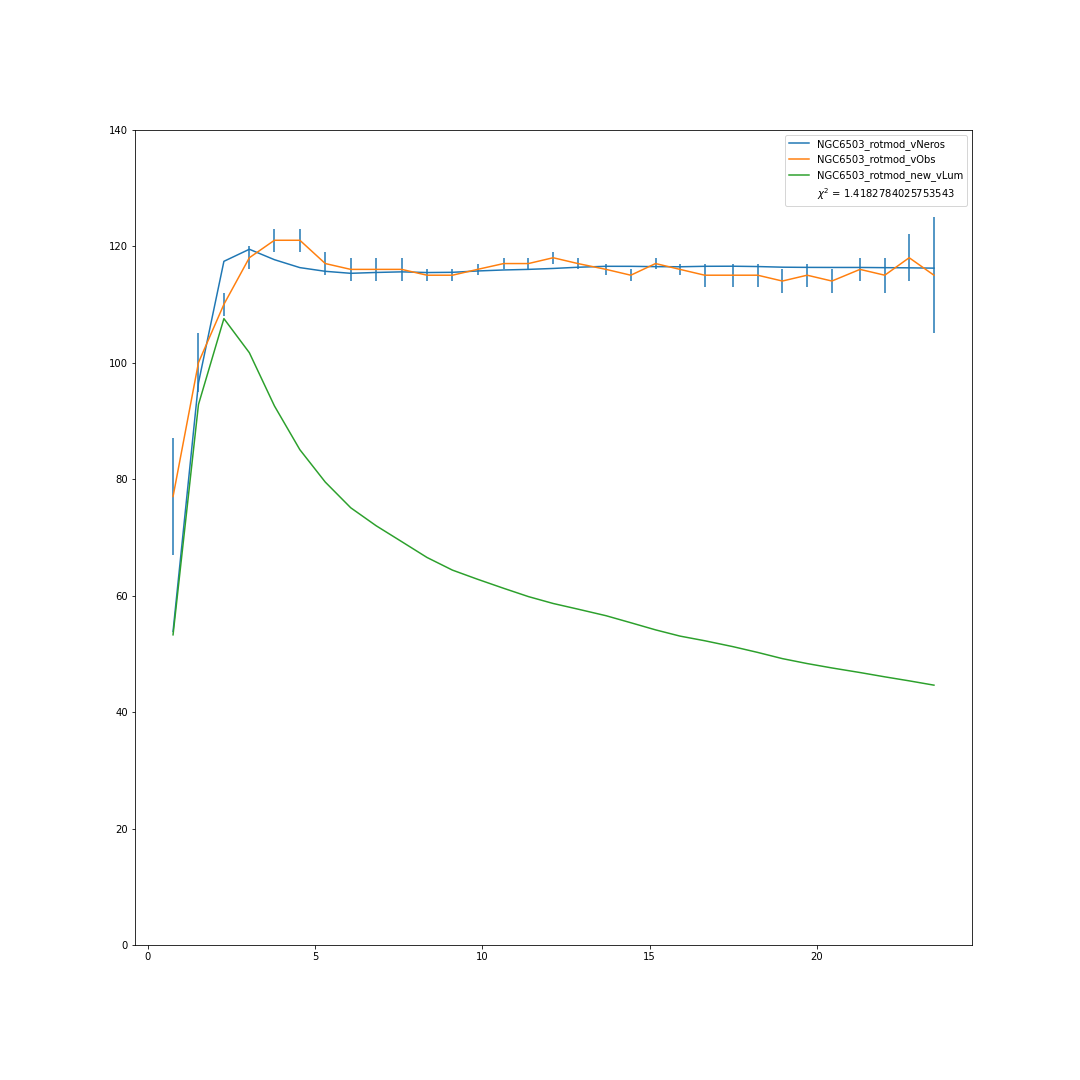
\includegraphics[width=0.95\linewidth]{figures/NGC6503_rotmod_XueSofue.png}
    \caption{Disk dominated NGC 6503} 
    \label{fig7:b} 
    \vspace{4ex}
  \end{subfigure} 
  \begin{subfigure}[c]{0.5\linewidth}
    \centering
    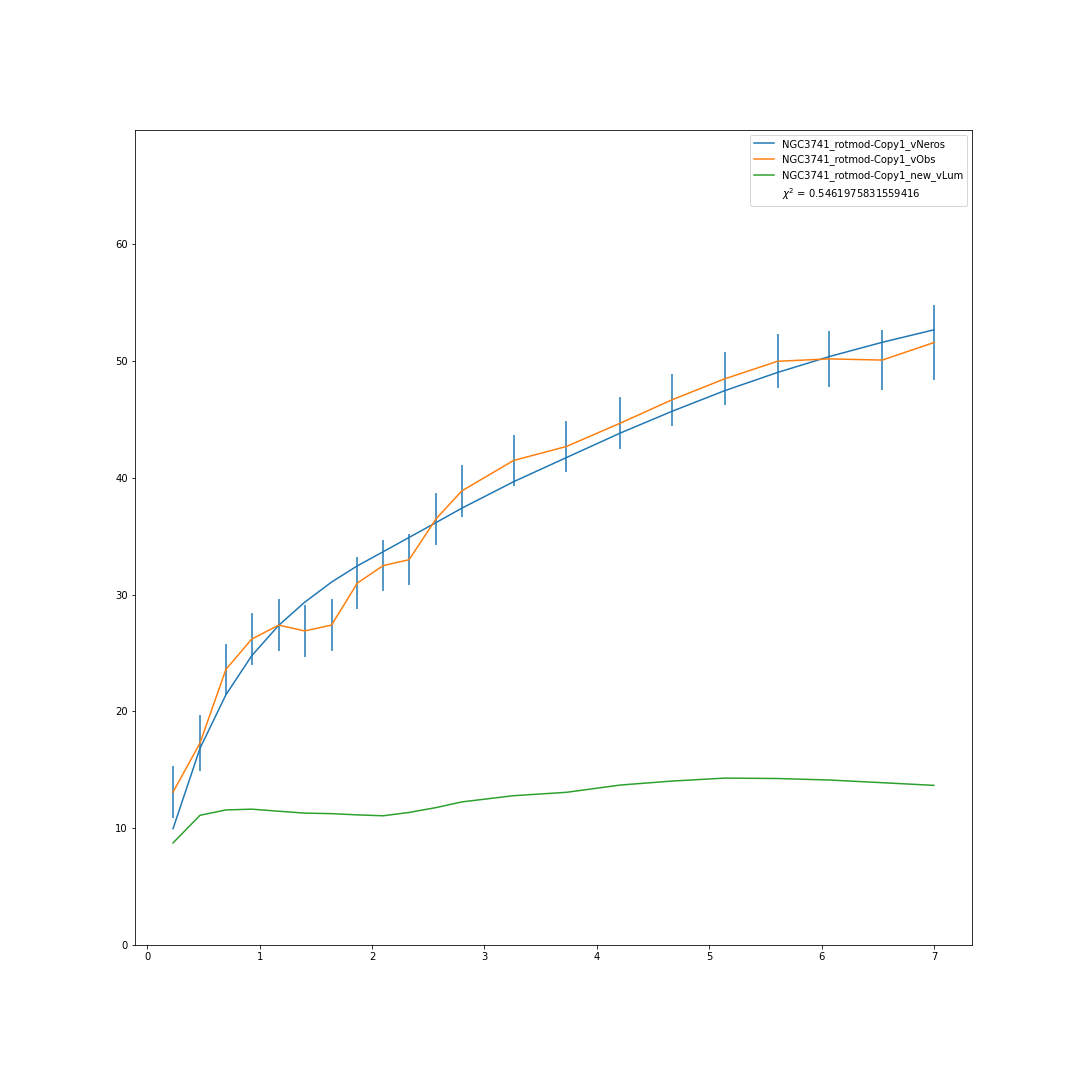
\includegraphics[width=0.95\linewidth]{figures/NGC3741_rotmod-Copy1_XueSofue.png} 
    \caption{Gas dominated NGC 3741} 
    \label{fig7:c} 
  \end{subfigure}%%
  \caption{Examples of range of spiral galaxy densities and RCFM rotation curve fits, points with error bars are the rotation curve data, Combined baryonic models are represented by the green lines, and the RCFM fit is the blue line. (YO BLUE : NOTE: remove orange lines, fit through data distracts from our fit)  }
  \label{fig7} 
\end{figure*}
 
 
    
%%%%%%%%%%%%%%%%%%%%%%%%%%%%%%%%%%%%%%%%%%%%%%%%%%%%%%%%%%%%%%%%%%%%%%%%%%%%%%%%%%%%%%%%%%%%%%%%%%%%%%%%%%%%%%%%%%%%%%%%%%%%%%%%%%%%%%%%%%%%%%%%%%%%%%%%%%%%%%%%%%%%%%%%%%%%%%%%%%%%%%%%%%%%%%%%%%%%%%%%%%%%%%%%%%%%%%%%%%%%%%%%%%%%%%%%%%%%%%%%%%%%%%%%%%%%%%%%%%%%%%%%%%%%%%%%%%%%%%%%%%%%%%%%%%%%%%%%%%%%%%%%%%%%%%%%%%%%%%%%%%%%%%%%%%%%%%%%%%%%%%%%  
    
     

\bibliography{LCM} 

\end{document}
%
% ****** End of file apssamp.tex ******